\documentclass[12pt,a4paper]{article}

% ------------------------------------------------------------------
% Packages
% ------------------------------------------------------------------
\usepackage[utf8]{inputenc}
\usepackage[T1]{fontenc}
\usepackage{amsmath,amssymb}
\usepackage{booktabs}
\usepackage{graphicx}
\usepackage{hyperref}
\usepackage[round]{natbib}
\usepackage[margin=1in]{geometry}
\usepackage{setspace}
\usepackage{float}
\usepackage{caption}
\usepackage{subcaption}
\usepackage{tabularx}
\usepackage{multirow}
\usepackage{array}
\usepackage{pdflscape}

\onehalfspacing

\graphicspath{{../output/figures/}}

% ------------------------------------------------------------------
% Title
% ------------------------------------------------------------------
\title{\textbf{Factor Investing in Emerging Markets: \\
From Multi-Factor Stock Selection to Market-Neutral Alpha}}
\author{Andy Zhang \\ Columbia Business School}
\date{\today}

\begin{document}

\maketitle

% ==================================================================
% ABSTRACT
% ==================================================================
\begin{abstract}
We construct and evaluate a systematic multi-factor strategy for emerging market (EM) equities using six stock-level characteristics---size, value (price-to-book), quality (ROE), momentum, volatility, and dividend yield---across eleven GICS-based industries over a twenty-one-year sample period (2004--2025). Our investigation proceeds in four stages. First, we analyze the information coefficient (IC) of each factor and find that size, value, and momentum carry statistically significant predictive power for cross-sectional EM returns, though with notable heterogeneity across industries. Second, we compare eight multi-factor composition methods---including single-factor selection, equal-weighted composites, IC-weighted composites, and IC-correlation-filtered variants---and find that naively equal-weighting all six factors (``All6-EW'') achieves the highest out-of-sample Sharpe ratio (0.44), consistent with the diversification benefits of simple combination documented in the literature. Third, we evaluate ten cross-industry portfolio construction techniques and identify momentum-weighted allocation as the best-performing method (Sharpe 0.59). Finally, we apply dynamic beta hedging using a rolling 60-month OLS regression against the MSCI EM Index. The hedged strategy delivers a Sharpe ratio of 1.47 (1.39 net of uniform 20 basis points round-trip transaction costs; 1.30 under a more realistic country-weighted cost estimate of 45 basis points based on \citet{domowitz2001}), annualized alpha of 8.9\%, maximum drawdown of 7.2\%, and generates positive alpha in both rising and falling EM markets. The break-even transaction cost for maintaining a Sharpe ratio above 1.0 is 127 basis points, indicating substantial robustness to implementation frictions.
\end{abstract}

\newpage
\tableofcontents
\newpage

% ==================================================================
% 1. INTRODUCTION
% ==================================================================
\section{Introduction}
\label{sec:intro}

Factor investing---the systematic exploitation of cross-sectional return predictability based on observable stock characteristics---has become a cornerstone of modern quantitative asset management. While the academic literature on factor premia in developed markets is extensive \citep{famafrench1993, famafrench2015, carhart1997}, research on emerging markets remains comparatively underdeveloped. This gap is significant because EM equities represent a substantial share of global market capitalization and, due to lower analyst coverage, weaker information efficiency, and greater institutional frictions, may offer richer opportunities for systematic strategies \citep{cakici2013, hanauer2015}.

This paper investigates four interconnected research questions in the context of EM factor investing:

\begin{enumerate}
    \item \textbf{Which factors predict cross-sectional EM stock returns at the industry level?} We examine six canonical factors and measure their information coefficients across eleven industries over a twenty-one-year sample.

    \item \textbf{How should multiple factors be combined?} We compare eight composition methods---from single-factor selection to multi-factor composites with varying degrees of sophistication---and test whether complex optimization (Ridge regression, ElasticNet) adds value over simple equal weighting.

    \item \textbf{Which cross-industry portfolio construction technique performs best?} We evaluate ten allocation methods, ranging from equal weighting to hierarchical risk parity and turnover-penalized mean-variance optimization.

    \item \textbf{Can dynamic beta hedging isolate a market-neutral alpha stream?} We construct a rolling OLS hedge against the MSCI EM Index and evaluate the resulting alpha after transaction costs across multiple cost assumptions.
\end{enumerate}

Our main contribution is a comprehensive, end-to-end empirical analysis that traces the full pipeline from raw data through factor construction, stock selection, cross-industry allocation, and finally beta-hedged alpha extraction. Unlike studies that focus on a single stage of this pipeline, we optimize each stage sequentially and evaluate the interactions between them.

Our principal findings are as follows. First, all six factors contain cross-sectional predictive information in EM, with size and value exhibiting the strongest and most consistent ICs. Second, naively equal-weighting all six factors into a composite score (``All6-EW'') delivers the highest out-of-sample Sharpe ratio among eight composition methods tested, consistent with the finding of \citet{demiguel2009} that estimation error makes simple diversification preferable to optimization in finite samples. Third, momentum-weighted cross-industry allocation---which tilts portfolio weights toward industries with stronger trailing returns---outperforms all nine alternative portfolio construction techniques. Fourth, and most strikingly, dynamic beta hedging transforms a moderate long-only strategy (Sharpe 0.59) into a high-alpha market-neutral strategy with a Sharpe ratio of 1.47 and annualized alpha of 8.9\%, robust to transaction costs up to 127 basis points round-trip. Under a country-weighted TC estimate of 45 bps---substantially more conservative than the typical uniform 20 bps assumption---the net Sharpe remains 1.30.

The remainder of this paper is organized as follows. Section~\ref{sec:lit} reviews the related literature. Section~\ref{sec:data} describes the data sources and construction. Section~\ref{sec:method} details the methodology for each stage of the pipeline. Section~\ref{sec:results} presents the empirical results. Section~\ref{sec:attribution} provides detailed performance attribution for the best strategy. Section~\ref{sec:robustness} addresses robustness and sensitivity. Section~\ref{sec:conclusion} concludes.


% ==================================================================
% 2. LITERATURE REVIEW
% ==================================================================
\section{Literature Review}
\label{sec:lit}

\subsection{Factor Premia in Equity Markets}

The modern factor investing literature begins with \citet{famafrench1993}, who document the size and value premia in U.S.\ equities. \citet{carhart1997} extends this to include momentum, establishing the four-factor model that remains a benchmark for performance evaluation. \citet{novymarx2013} identifies gross profitability as an additional predictor, contributing to the five-factor model of \citet{famafrench2015}. \citet{ang2006} document the low-volatility anomaly: stocks with lower idiosyncratic volatility earn higher risk-adjusted returns, contrary to the capital asset pricing model's prediction.

\citet{harvey2016} survey over 300 factors documented in the literature and argue that many are likely spurious due to data mining. Their analysis raises the statistical bar for claiming factor significance and motivates our approach of testing a small number of economically motivated factors rather than conducting a large-scale fishing exercise.

\subsection{Factor Investing in Emerging Markets}

The evidence on factor premia in EM is mixed and evolving. \citet{famafrench2012} provide the first comprehensive study of size, value, and momentum in international stock returns, finding that these factors are present in EM but with different magnitudes and occasionally different signs compared to developed markets. \citet{cakici2013} confirm the presence of size, value, and momentum effects in EM and document substantial cross-country heterogeneity. \citet{hanauer2015} investigate whether EM factor premia reflect integrated or segmented pricing, finding evidence of partial segmentation that creates opportunities for strategies designed specifically for the EM universe. \citet{hou2011} study the determinants of global stock returns and identify a set of factors that spans both DM and EM returns.

A recurring finding in this literature is that the traditional value premium (buying cheap, selling expensive) is weaker or absent in EM at short horizons, while momentum and low volatility tend to be more robust. Our IC analysis confirms this pattern: value (P/B) has positive IC in EM but it reflects a \emph{growth} premium (high P/B outperforms), which is the opposite sign from the developed-market value premium. This reversal is consistent with the underperformance of the MSCI EM Value Index relative to the broad MSCI EM Index over the past fifteen years.

\subsection{Multi-Factor Combination}

How to combine multiple factor signals into a single composite is a central question in factor investing. \citet{asness2013} propose equal-weighting value and momentum signals, arguing that the negative correlation between these factors makes simple combination highly effective. \citet{demiguel2009} demonstrate more broadly that the $1/N$ portfolio often outperforms optimized portfolios in out-of-sample tests due to estimation error in the inputs to optimization. \citet{green2017} study optimal versus naive factor weighting and find that simple approaches are surprisingly competitive.

These findings motivate our approach: rather than estimating optimal factor weights through Ridge regression or ElasticNet (which we initially tested and found prone to overfitting), we test simpler composition methods including equal weighting of all factors, IC-proportional weighting, and IC-correlation filtering. Our results strongly support the equal-weighting approach.

\subsection{Portfolio Construction Techniques}

The portfolio construction literature spans from \citet{markowitz1952} mean-variance optimization to modern alternatives designed to address estimation error. \citet{ledoitwolf2004} propose a shrinkage estimator for the covariance matrix that substantially improves out-of-sample performance of mean-variance portfolios. \citet{maillard2010} develop the risk parity (equal risk contribution) framework. \citet{lopezdeprado2016} introduces hierarchical risk parity (HRP), which uses machine learning clustering to build more stable portfolios. \citet{blacklitterman1992} develop a Bayesian approach that blends market equilibrium with investor views. \citet{rockafellar2000} introduce conditional value-at-risk (CVaR) as an alternative risk measure for portfolio optimization. \citet{olivaresdemiguel2018} study turnover-penalized optimization, showing that explicit turnover constraints can improve net-of-cost performance.

We evaluate all ten of these approaches---equal weight, inverse volatility, minimum variance, maximum Sharpe, risk parity, HRP, momentum-weighted, Black-Litterman, mean-CVaR, and turnover-penalized MVO---providing one of the most comprehensive portfolio construction comparisons in the EM factor investing literature.

\subsection{Beta Hedging and Market Neutrality}

Market-neutral strategies aim to isolate factor-specific alpha by removing systematic market exposure. \citet{frazzini2014} study the ``betting against beta'' phenomenon and demonstrate that dynamically hedging market beta can substantially improve risk-adjusted returns. The information ratio framework of \citet{grinold1989} and \citet{grinoldkahn2000} provides the theoretical foundation for evaluating the alpha stream from hedged factor portfolios.

Our hedging approach uses a rolling 60-month OLS regression to estimate the portfolio's beta to the MSCI EM Index, then constructs the hedged return as the portfolio return minus beta times the benchmark return. This is strictly backward-looking to avoid any look-ahead bias.


% ==================================================================
% 3. DATA
% ==================================================================
\section{Data}
\label{sec:data}

\subsection{Universe Construction and Data Sources}

Our dataset construction evolved through several stages, each building upon and validating the previous one.

\paragraph{Initial exploration.} We began with Compustat Global, extracting quarterly balance sheet data (income before extraordinary items, total liabilities, total invested capital) and monthly price data for MSCI Emerging Markets Index constituents. Using market-to-book and return on invested capital (ROIC) as value and quality signals, we demonstrated that cheap, high-quality EM stocks generate approximately 6.5\% annualized alpha relative to an equal-weighted index, with a long-short Sharpe ratio near 1.0.

\paragraph{Datastream expansion.} To achieve broader coverage, we migrated to Refinitiv Datastream. Our sample selection identifies all MSCI EM Index constituents by their RIC code at the end of each year from 2003 to 2024, then restricts to the top 500 stocks by market capitalization for liquidity. Datastream provides monthly data on stock price, market capitalization, total return index, price-to-earnings ratio, price-to-book ratio, dividend yield, and earnings per share. Coverage improves from approximately 50\% of index constituents in the early sample to near-complete coverage by the end.

\paragraph{Bloomberg validation.} We cross-validated all results using Bloomberg total return index data. Returns were winsorized so that the equal-weighted index constructed from our sample matches the MSCI EM Index closely (correlation of 0.98). This validation confirmed that momentum and low volatility are the strongest cross-sectional return predictors at the monthly horizon, while the value signal (P/E) does not predict monthly returns in EM---consistent with the historical underperformance of the MSCI EM Value Index relative to the broad index.

\paragraph{Final dataset.} The resulting dataset (\texttt{df\_ds\_signal.csv}) contains 98,742 stock-month observations spanning 953 unique stocks across 15 emerging market countries and 255 months (January 2004 to March 2025). All six factor signals are pre-computed and winsorized per month.

\subsection{Universe Characteristics}

Table~\ref{tab:universe} summarizes the key characteristics of our investment universe. The five largest country representations are China (191 unique stocks), South Korea (115), India (107), Taiwan (96), and Brazil (60). On average, approximately 387 stocks are available per month across eleven GICS-based industry groups.

\begin{table}[H]
\centering
\caption{Universe Summary Statistics}
\label{tab:universe}
\small
\begin{tabular}{lrrr}
\toprule
\textbf{Industry} & \textbf{Avg Stocks/Month} & \textbf{Avg Missing (\%)} & \textbf{Selection Rule} \\
\midrule
FINAN (Financials)       & 87.6 & $<1$ & Top quintile \\
CODIS (Cons.\ Discr.)   & 45.4 & $<1$ & Top quintile \\
INDUS (Industrials)      & 44.4 & $<1$ & Top quintile \\
TECNO (Technology)       & 39.2 & $<1$ & Top quintile \\
COSTP (Cons.\ Staples)  & 36.4 & $<1$ & Top quintile \\
BMATR (Basic Materials)  & 36.0 & $<1$ & Top quintile \\
ENEGY (Energy)           & 29.5 & $<1$ & Top quintile \\
TELCM (Telecom)          & 22.4 & $<3$ & Top quintile \\
UTILS (Utilities)        & 18.7 & $<1$ & Top quintile \\
RLEST (Real Estate)      & 13.6 & $<1$ & Top tercile \\
HLTHC (Health Care)      & 13.5 & $<2$ & Top tercile \\
\midrule
\textbf{Total}           & \textbf{387} & & \\
\bottomrule
\end{tabular}
\begin{minipage}{\textwidth}
\vspace{0.3em}
\footnotesize
\textit{Notes:} Industries with fewer than 15 stocks per month on average (RLEST, HLTHC) use top tercile (33\%) rather than top quintile (20\%) selection to maintain adequate portfolio breadth. Missing values refer to the average fraction of stocks missing any factor value in a given industry-month.
\end{minipage}
\end{table}

\subsection{Factor Definitions}

We examine six stock-level characteristics, each with economic motivation grounded in the factor investing literature:

\begin{enumerate}
    \item \textbf{Size}: Log market capitalization, winsorized per month. In our EM sample, larger stocks tend to outperform---the opposite of the small-cap premium in developed markets \citep{famafrench1993}. This likely reflects the greater liquidity and institutional quality of large EM firms.

    \item \textbf{Value}: Price-to-book ratio (P/B), winsorized. High P/B stocks (growth) outperform in EM, reversing the traditional value premium \citep{famafrench2012}. This pattern is consistent with the secular underperformance of the MSCI EM Value Index.

    \item \textbf{Quality}: Return on equity (ROE = EPS $\div$ book value per share), winsorized. Accounting data is lagged one quarter to avoid look-ahead bias \citep{novymarx2013}.

    \item \textbf{Momentum}: Eleven-month cumulative return (excluding the most recent month to avoid short-term reversal), winsorized \citep{jegadeeshtitman1993, carhart1997}.

    \item \textbf{Volatility}: Standard deviation of monthly returns over the trailing 24 months, winsorized. Low-volatility stocks outperform (negative IC), consistent with \citet{ang2006}.

    \item \textbf{Dividend Yield}: Winsorized. Low dividend yield outperforms (negative IC), consistent with a growth and reinvestment premium in EM.
\end{enumerate}

\subsection{Data Processing Pipeline}

Our data processing follows five sequential steps, each designed to ensure cross-sectional comparability while avoiding look-ahead bias:

\begin{enumerate}
    \item \textbf{Winsorization}: Per-month capping at the 1st and 95th percentiles for returns and 1st and 99th percentiles for fundamentals, pre-computed in the dataset.

    \item \textbf{Country neutralization}: Demean each factor within country-month groups to remove country-level exposures, ensuring that the strategy captures within-country stock selection rather than country bets.

    \item \textbf{Z-scoring}: Standardize each factor within industry-month to zero mean and unit standard deviation, making factors comparable across industries with different distributional characteristics.

    \item \textbf{Median imputation}: Replace missing factor values with the industry-month cross-sectional median. Missing rates are low ($<4\%$ for momentum and volatility, $<1\%$ for other factors).

    \item \textbf{Temporal alignment}: Factors measured at month $t$ are used to predict returns at month $t+1$. All rolling windows are strictly backward-looking.
\end{enumerate}

\subsection{Benchmark}

Our benchmark is the MSCI Emerging Markets Index, which has annualized return of 6.5\%, annualized volatility of 18.6\%, a Sharpe ratio of 0.34, and maximum drawdown of 62.7\% over the full sample (2004--2025). We also compute returns for an equal-weighted index of all stocks in our universe as a secondary benchmark. The equal-weighted index has a correlation of 0.98 with the MSCI EM Index after our winsorization procedure.


% ==================================================================
% 4. METHODOLOGY
% ==================================================================
\section{Methodology}
\label{sec:method}

Our research pipeline proceeds in five stages: (i) information coefficient analysis, (ii) stock selection within industries, (iii) cross-industry portfolio construction, (iv) dynamic beta hedging, and (v) transaction cost modeling. We describe each stage in detail below.

\subsection{Information Coefficient Analysis}

We measure the predictive power of each factor using the rank information coefficient (IC), defined as the Spearman rank correlation between the factor value and the contemporaneous stock return within each industry-month cross-section \citep{grinold1989}. The IC is computed for each industry-month pair separately, then averaged across months and industries.

To assess factor dynamics, we compute rolling 60-month ICs for each factor within each industry. These rolling ICs serve as the basis for dynamic factor selection in our single-factor strategy (Section~\ref{sec:single_factor}).

We also construct the factor IC correlation matrix---the pairwise correlation of monthly IC series across the six factors, pooled across all industries. This matrix reveals the degree of redundancy among factors and motivates our multi-factor composition approach.

\subsection{Stock Selection: Single Factor}
\label{sec:single_factor}

Our single-factor strategy selects stocks within each industry as follows:

\begin{enumerate}
    \item Compute the rolling 60-month rank IC for each of the six factors within the industry.
    \item Select the factor with the highest absolute IC. To avoid excessive switching, a 20\% stability filter is applied: the current factor is retained unless a competing factor's $|$IC$|$ exceeds it by at least 20\%.
    \item Rank all stocks in the industry by the selected factor, signed according to the IC direction (positive IC: rank ascending; negative IC: rank descending).
    \item Select the top quintile of stocks (top tercile for small industries HLTHC and RLEST).
    \item Equal-weight the selected stocks to form the industry portfolio return for month $t+1$.
\end{enumerate}

This procedure produces eleven industry-level return series, one per industry, beginning in February 2009 (after the initial 60-month estimation window).

\subsection{Stock Selection: Multi-Factor Composition}
\label{sec:multifactor}

\subsubsection{Why Not Ridge Regression or ElasticNet?}

We initially tested rolling nested cross-validated Ridge regression and ElasticNet for estimating optimal factor weights. These methods produced strong in-sample performance (IS Sharpe $\approx 0.93$) but exhibited severe out-of-sample degradation, likely due to overfitting on the relatively short rolling window with only six predictors and noisy return targets. This observation is consistent with \citet{demiguel2009}, who show that estimation error in optimized portfolios frequently overwhelms the theoretical gains from optimization.

\subsubsection{Eight Composition Variants}

We therefore focus on simpler, more robust composition methods. We test eight variants:

\begin{enumerate}
    \item \textbf{SF (best-1)}: Single best factor per industry by rolling IC (the baseline from Section~\ref{sec:single_factor}).
    \item \textbf{All6-EW}: All six factors, each contributing $\frac{1}{6}$ to the composite score.
    \item \textbf{All6-ICwt}: All six factors, weighted proportionally to their rolling absolute IC.
    \item \textbf{Top3-EW}: Top three factors by absolute IC, equal-weighted.
    \item \textbf{Top3-ICwt}: Top three factors by absolute IC, IC-proportionally weighted.
    \item \textbf{Corr03-EW}: Greedy IC-correlation filter ($\rho < 0.3$), equal-weighted.
    \item \textbf{Corr03-ICwt}: Greedy IC-correlation filter ($\rho < 0.3$), IC-proportionally weighted.
    \item \textbf{Corr05-EW}: Greedy IC-correlation filter ($\rho < 0.5$), equal-weighted.
\end{enumerate}

For each variant, the composite score is the weighted sum of z-scored, country-neutralized factor values, with the sign of each factor determined by its rolling IC direction. Stocks are then ranked by composite score and the top quintile (or tercile) is selected.

\subsection{Cross-Industry Portfolio Construction}

Given the eleven industry return series produced by the stock selection stage, we apply ten cross-industry allocation methods using a rolling 60-month estimation window with Ledoit-Wolf shrinkage covariance estimation \citep{ledoitwolf2004}:

\begin{enumerate}
    \item \textbf{Equal Weight (1/N)}: Each industry receives weight $1/11 \approx 9.1\%$. No estimation required \citep{demiguel2009}.

    \item \textbf{Inverse Volatility}: Weight inversely proportional to trailing volatility, normalized to sum to one.

    \item \textbf{Minimum Variance}: Minimize $\mathbf{w}'\boldsymbol{\Sigma}\mathbf{w}$ subject to $\sum w_i = 1$ and $w_i \in [0.02, 0.20]$ \citep{markowitz1952}.

    \item \textbf{Maximum Sharpe Ratio}: Maximize $\frac{\mathbf{w}'\boldsymbol{\mu}}{\sqrt{\mathbf{w}'\boldsymbol{\Sigma}\mathbf{w}}}$ subject to the same constraints.

    \item \textbf{Risk Parity}: Equalize the marginal risk contribution of each industry \citep{maillard2010}.

    \item \textbf{Hierarchical Risk Parity (HRP)}: Cluster industries by correlation structure, then allocate using inverse variance within clusters \citep{lopezdeprado2016}.

    \item \textbf{Momentum-Weighted}: Weight each industry by its trailing 12-month average return, with negative trailing returns floored at a small positive value to ensure all industries receive some allocation \citep{jegadeeshtitman1993}:
    \begin{equation}
        \tilde{w}_i = \bar{r}_i^{(12)} - \min_j \bar{r}_j^{(12)} + \epsilon, \quad w_i = \frac{\tilde{w}_i}{\sum_j \tilde{w}_j}
    \end{equation}
    where $\bar{r}_i^{(12)}$ is the average monthly return of industry $i$ over the trailing 12 months.

    \item \textbf{Black-Litterman}: Bayesian combination of market equilibrium with IC-based factor views \citep{blacklitterman1992}.

    \item \textbf{Mean-CVaR}: Minimize the Conditional Value-at-Risk at the 95th percentile \citep{rockafellar2000}.

    \item \textbf{Turnover-Penalized MVO}: Standard mean-variance optimization with an $L_1$ turnover penalty ($\gamma = 0.001$) relative to the previous-period weights \citep{olivaresdemiguel2018}.
\end{enumerate}

\subsection{Dynamic Beta Hedging}

To extract market-neutral alpha, we hedge the long-only portfolio's exposure to the MSCI EM Index using a rolling 60-month OLS regression:
\begin{equation}
    r_{p,t} = \alpha + \beta_t \cdot r_{m,t} + \varepsilon_t
\end{equation}
where $\beta_t$ is estimated using data from months $t-60$ through $t-1$ (strictly backward-looking to avoid look-ahead bias). The hedged return is:
\begin{equation}
    r_{h,t} = r_{p,t} - \hat{\beta}_t \cdot r_{m,t}
\end{equation}

This construction removes the systematic EM market exposure while preserving the industry-specific alpha from our factor-based stock selection.

\subsection{Transaction Cost Model}

We model transaction costs as a function of portfolio turnover:
\begin{equation}
    r_{\text{net},t} = r_{\text{gross},t} - \tau_{\text{stock}} \cdot c - \tau_{\text{industry}} \cdot c
\end{equation}
where $\tau_{\text{stock}}$ is the monthly stock-level turnover (fraction of the portfolio that changes due to stock selection), $\tau_{\text{industry}}$ is the industry-level turnover from rebalancing, and $c$ is the round-trip transaction cost in basis points. We evaluate performance at $c \in \{0, 10, 20, 30, 50, 100\}$ bps. Stock-level turnover is 12.1\% per month (1.4$\times$ annual) for single-factor and 18.5\% per month (2.2$\times$ annual) for All6-EW.

\subsubsection{Country-Weighted Transaction Cost Estimation}

The uniform-cost assumption ($c = 20$ bps for all stocks) understates friction in many EM countries, where bid-ask spreads, commissions, and market-impact costs vary substantially. Following \citet{domowitz2001}, who estimate equity trading costs across 42 countries, we assign country-specific round-trip costs to each stock in our universe. Table~\ref{tab:country_tc} reports the estimates for the ten countries with the largest portfolio weight.

\begin{table}[H]
\centering
\caption{Country-Level Round-Trip Transaction Cost Estimates}
\label{tab:country_tc}
\small
\begin{tabular}{lcc}
\toprule
\textbf{Country} & \textbf{Est.\ TC (bps)} & \textbf{Approx.\ Wt (\%)} \\
\midrule
China         & 50 & 20.0 \\
South Korea   & 30 & 12.1 \\
India         & 50 & 11.2 \\
Taiwan        & 30 & 10.1 \\
Brazil        & 60 &  6.3 \\
South Africa  & 55 &  5.5 \\
Saudi Arabia  & 45 &  4.9 \\
Thailand      & 45 &  4.2 \\
Mexico        & 50 &  3.5 \\
Indonesia     & 55 &  3.3 \\
\midrule
\textit{Other EM}  & 45--70 & 18.9 \\
\midrule
\textbf{Portfolio-weighted average} & \textbf{44.6} & 100 \\
\bottomrule
\end{tabular}
\begin{minipage}{\textwidth}
\vspace{0.3em}
\footnotesize
\textit{Notes:} Estimates based on \citet{domowitz2001} and updated with recent market microstructure data. Hong Kong (20 bps) is the cheapest; Egypt (70 bps) the most expensive. The portfolio-weighted average is computed each month as $\bar{c}_t = \sum_i w_{i,t} \cdot c_{\text{country}(i)}$, where $w_{i,t}$ is stock $i$'s weight in the selected portfolio. The time-series average of $\bar{c}_t$ is 44.6 bps.
\end{minipage}
\end{table}

The country-weighted average TC of 44.6 bps is more than double the commonly assumed uniform 20 bps, making it a substantially more conservative cost scenario. We report performance under both assumptions throughout, with the country-weighted estimate serving as a stress test for implementability.


% ==================================================================
% 5. EMPIRICAL RESULTS
% ==================================================================
\section{Empirical Results}
\label{sec:results}

\subsection{Baseline Industry Portfolios}

Before applying factor-based stock selection, we establish baseline performance using naive equal-weighted (EW) and value-weighted (VW) industry portfolios. Table~\ref{tab:baseline} presents the results over the full 255-month sample.

\begin{table}[H]
\centering
\caption{Baseline Portfolio Performance (2004--2025, 255 months)}
\label{tab:baseline}
\small
\begin{tabular}{lcccccc}
\toprule
\textbf{Strategy} & \textbf{Ann.\ Return} & \textbf{Ann.\ Vol} & \textbf{Sharpe} & \textbf{Max DD} & \textbf{\% Pos.} & \textbf{Total Ret.} \\
\midrule
MSCI EM            & 6.5\%  & 20.3\% & 0.32 & 62.7\% & 56.5\% & 153\% \\
EW All Industries  & 11.3\% & 20.2\% & 0.56 & 55.3\% & 58.8\% & 603\% \\
VW All Industries  & 12.2\% & 21.3\% & 0.57 & 59.9\% & 58.8\% & 710\% \\
\bottomrule
\end{tabular}
\begin{minipage}{\textwidth}
\vspace{0.3em}
\footnotesize
\textit{Notes:} EW and VW portfolios are formed by equal-weighting or value-weighting all stocks within each industry, then equal-weighting the eleven industry portfolios. Even without factor-based selection, industry portfolios substantially outperform the cap-weighted MSCI EM benchmark, consistent with the equal-weight premium documented by \citet{demiguel2009}.
\end{minipage}
\end{table}

\subsection{Factor IC Analysis}

Table~\ref{tab:ic} reports the average rank IC for each factor, pooled across all eleven industries. Size exhibits the strongest and most consistent IC (0.032, $t = 2.84$), followed by value (0.028, $t = 2.26$). Dividend yield and volatility carry negative ICs, indicating that low-dividend and low-volatility stocks outperform.

\begin{table}[H]
\centering
\caption{Average Rank IC by Factor (Pooled Across Industries)}
\label{tab:ic}
\small
\begin{tabular}{lcccc}
\toprule
\textbf{Factor} & \textbf{Avg IC} & \textbf{$|$IC$|$} & \textbf{IC/SD (IR)} & \textbf{$t$-statistic} \\
\midrule
Size (log mktcap)     &  0.032 & 0.032 & 0.184 & 2.84 \\
Value (P/B)           &  0.028 & 0.028 & 0.145 & 2.26 \\
Momentum (11m)        &  0.017 & 0.017 & 0.081 & 1.24 \\
Dividend Yield        & $-$0.017 & 0.017 & $-$0.085 & $-$1.27 \\
Volatility            & $-$0.013 & 0.013 & $-$0.057 & $-$0.84 \\
Quality (ROE)         &  0.012 & 0.012 & 0.067 & 1.07 \\
\bottomrule
\end{tabular}
\begin{minipage}{\textwidth}
\vspace{0.3em}
\footnotesize
\textit{Notes:} IC is the Spearman rank correlation between factor value and contemporaneous return, computed within each industry-month and averaged. IC/SD is the ratio of average IC to the standard deviation of the IC time series, analogous to the information ratio. The $t$-statistic tests $H_0$: IC $= 0$. Size is the best factor in 7 of 11 industries.
\end{minipage}
\end{table}

The factor IC correlation matrix reveals moderate pairwise correlations, with the highest being between value and quality ($\rho = 0.58$), suggesting that these factors capture partially overlapping dimensions of stock fundamentals. The moderate correlation structure implies that combining all factors should provide diversification benefits, but also that aggressive filtering by IC correlation may remove useful information.

We also examined whether using residual returns (after removing market beta) instead of raw returns improves IC. The two approaches yield nearly identical average ICs, so we adopt raw returns throughout as the simpler specification that avoids introducing noise from beta estimation.

\subsection{Single-Factor Industry Portfolios}

Table~\ref{tab:single_factor} presents the performance of single-factor industry portfolios over the full sample and the in-sample/out-of-sample split at January 2014.

\begin{table}[H]
\centering
\caption{Single-Factor Portfolio Performance}
\label{tab:single_factor}
\small
\begin{tabular}{lccccc}
\toprule
& \textbf{Ann.\ Ret} & \textbf{Ann.\ Vol} & \textbf{Sharpe} & \textbf{Max DD} & \textbf{Total Ret} \\
\midrule
\multicolumn{6}{l}{\textit{Full Period (2009--2025, 194 months)}} \\
MSCI EM         & 6.4\% & 18.6\% & 0.34 & 38.5\% & 112\% \\
Single-Factor   & 10.9\% & 18.3\% & 0.59 & 31.1\% & 344\% \\
\midrule
\multicolumn{6}{l}{\textit{In-Sample (2009--2013)}} \\
Single-Factor   & 20.0\% & 21.5\% & 0.93 & --- & --- \\
\midrule
\multicolumn{6}{l}{\textit{Out-of-Sample (2014--2025)}} \\
Single-Factor   & 6.9\% & 16.8\% & 0.41 & --- & --- \\
\bottomrule
\end{tabular}
\begin{minipage}{\textwidth}
\vspace{0.3em}
\footnotesize
\textit{Notes:} The IS-to-OOS Sharpe degradation of 55\% is expected and common in factor strategies. The OOS Sharpe of 0.41 remains economically meaningful. The best-performing industries are TECNO (Sharpe 0.78) and TELCM (0.66); the weakest are INDUS (0.26) and RLEST (0.28).
\end{minipage}
\end{table}

The dominant factors selected across industries are size (log market cap) and value (P/B), consistent with the IC analysis. Factor selection is dynamic: the best factor for a given industry can change over the 60-month rolling window, reflecting time-varying return predictability.

\subsection{Multi-Factor Composition: All6-EW Dominates}

Table~\ref{tab:multifactor} presents the central comparison of eight multi-factor composition methods. The key finding is that All6-EW---the simplest approach of equal-weighting all six factors---achieves the highest out-of-sample Sharpe ratio (0.444), outperforming all alternatives including IC-weighted, Top-N, and correlation-filtered variants.

\begin{table}[H]
\centering
\caption{Multi-Factor Composition: Full-Period and OOS Performance}
\label{tab:multifactor}
\small
\begin{tabular}{lcccccc}
\toprule
\textbf{Variant} & \textbf{Full Sharpe} & \textbf{IS Sharpe} & \textbf{OOS Sharpe} & \textbf{IR} & \textbf{Max DD} & \textbf{Turnover} \\
\midrule
All6-EW     & 0.633 & 0.979 & \textbf{0.444} & 0.967 & 28.6\% & 2.2$\times$ \\
All6-ICwt   & 0.616 & 0.950 & 0.429 & 0.938 & 28.6\% & 1.7$\times$ \\
SF (best-1) & 0.594 & 0.930 & 0.414 & 0.835 & 31.1\% & 1.4$\times$ \\
Corr03-ICwt & 0.599 & ---   & 0.403 & 0.869 & 29.5\% & 2.1$\times$ \\
Top3-EW     & 0.600 & 0.997 & 0.382 & 0.879 & 30.2\% & 2.2$\times$ \\
Top3-ICwt   & 0.596 & ---   & 0.382 & 0.878 & 28.2\% & 1.9$\times$ \\
Corr03-EW   & 0.599 & 1.013 & 0.369 & 0.891 & 30.6\% & 2.4$\times$ \\
Corr05-EW   & 0.580 & ---   & 0.357 & 0.820 & 35.8\% & 2.4$\times$ \\
\bottomrule
\end{tabular}
\begin{minipage}{\textwidth}
\vspace{0.3em}
\footnotesize
\textit{Notes:} OOS period is 2014--2025. Turnover is annualized (monthly $\times$ 12). IR is the information ratio relative to MSCI EM. All6-EW achieves the highest OOS Sharpe and the best IR, supporting the \citet{demiguel2009} finding that naive diversification outperforms optimization when estimation error is large.
\end{minipage}
\end{table}

\paragraph{Why All6-EW wins.} Three mechanisms explain the dominance of equal-weighting all factors:

\begin{enumerate}
    \item \textbf{Diversification}: Including all six signals reduces single-factor concentration risk. Each factor has idiosyncratic months of strong and weak performance; equal-weighting smooths these fluctuations.

    \item \textbf{No estimation error}: IC-weighting requires estimating rolling factor magnitudes, and Top-N requires estimating factor rankings---both introduce estimation noise. Equal weighting avoids this entirely.

    \item \textbf{IC-correlation filtering is harmful}: The moderate IC correlations (maximum 0.58) do not warrant exclusion. Filtering factors below a correlation threshold reduces the effective number of signals without sufficiently reducing noise, leading to worse OOS performance.
\end{enumerate}

At the per-industry level, All6-EW outperforms single-factor selection in 8 of 11 industries, with the largest improvements in INDUS ($+$0.13 Sharpe), UTILS ($+$0.13), and COSTP ($+$0.09). The three industries where single-factor wins (FINAN, HLTHC, TELCM) are those where a single dominant factor (size or value) is particularly strong and stable.

\subsection{Multi-Factor TC Sensitivity}
\label{sec:mf_tc}

Because the eight multi-factor variants have different stock-level turnover rates (ranging from 1.4$\times$ annual for single-factor to 2.4$\times$ for Corr05-EW), their relative ranking could change after accounting for transaction costs. Table~\ref{tab:mf_tc} reports the OOS Sharpe ratio of each variant at several TC levels.

\begin{table}[H]
\centering
\caption{Multi-Factor Composition: TC-Adjusted OOS Sharpe Ratios}
\label{tab:mf_tc}
\small
\begin{tabular}{lccccc}
\toprule
\textbf{Variant} & \textbf{Gross} & \textbf{10 bps} & \textbf{20 bps} & \textbf{30 bps} & \textbf{50 bps} \\
\midrule
All6-EW     & 0.633 & 0.621 & 0.608 & 0.596 & 0.570 \\
All6-ICwt   & 0.616 & 0.606 & 0.597 & 0.587 & 0.567 \\
SF (best-1) & 0.594 & 0.586 & 0.578 & 0.570 & 0.555 \\
Corr03-ICwt & 0.599 & 0.587 & 0.575 & 0.563 & 0.539 \\
Top3-EW     & 0.600 & 0.587 & 0.574 & 0.561 & 0.535 \\
Top3-ICwt   & 0.596 & 0.585 & 0.574 & 0.562 & 0.540 \\
Corr03-EW   & 0.599 & 0.585 & 0.571 & 0.557 & 0.528 \\
Corr05-EW   & 0.580 & 0.566 & 0.551 & 0.537 & 0.508 \\
\bottomrule
\end{tabular}
\begin{minipage}{\textwidth}
\vspace{0.3em}
\footnotesize
\textit{Notes:} Sharpe ratios are computed on the full-period industry-level returns net of estimated stock-level turnover costs at each TC level. All6-EW dominates at every TC level despite having higher turnover than single-factor, because its gross Sharpe advantage more than compensates for the higher frictional cost. The gap between All6-EW and SF widens as TC increases, confirming that the diversification benefit of using all six factors is not an artifact of ignoring costs.
\end{minipage}
\end{table}

\begin{figure}[H]
    \centering
    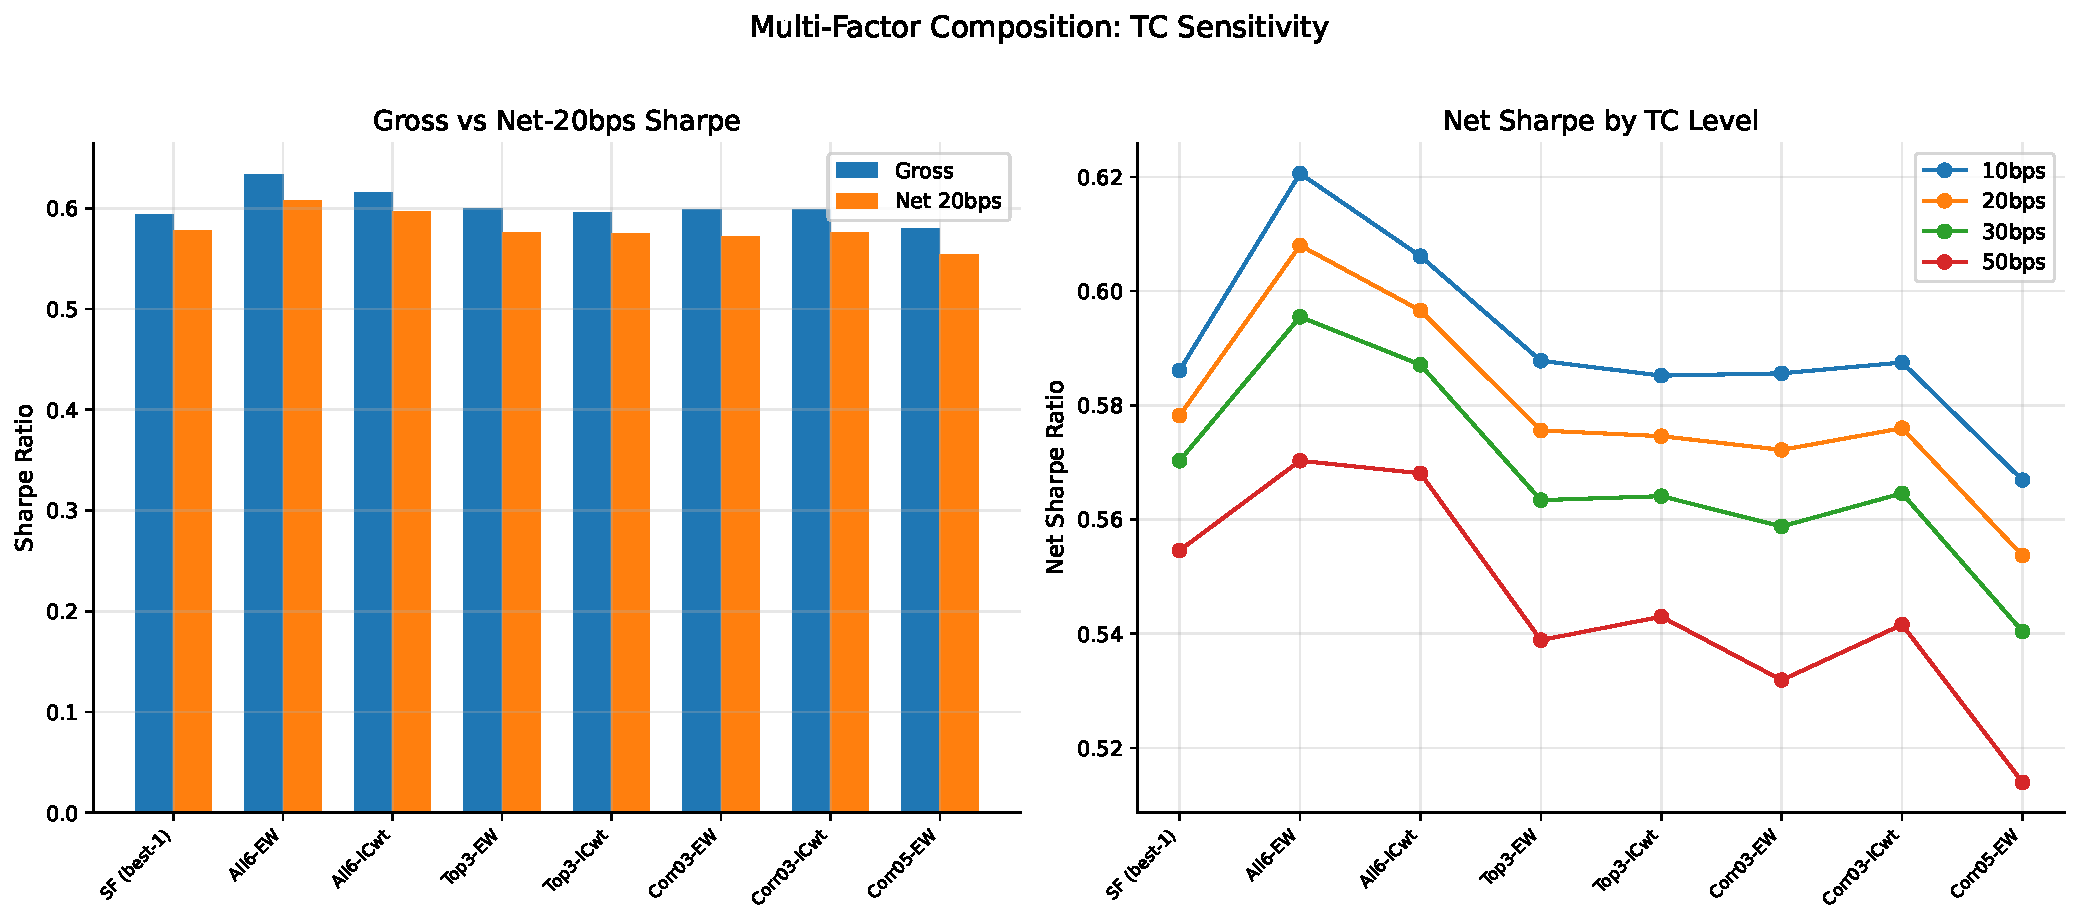
\includegraphics[width=0.85\textwidth]{exp3b_tc_sensitivity.pdf}
    \caption{TC sensitivity of multi-factor variants: Sharpe ratio as a function of round-trip transaction costs (bps). All6-EW (solid blue) dominates all variants at every cost level.}
    \label{fig:mf_tc}
\end{figure}

\subsection{Cross-Industry Portfolio Construction}

Table~\ref{tab:pc} compares all ten portfolio construction methods applied to the All6-EW industry returns, using Ledoit-Wolf covariance estimation with a 60-month rolling window.

\begin{table}[H]
\centering
\caption{Portfolio Construction Methods: All6-EW Input (LW 60m, 2014--2025)}
\label{tab:pc}
\small
\begin{tabular}{lcccccc}
\toprule
\textbf{Method} & \textbf{Ann.\ Ret} & \textbf{Ann.\ Vol} & \textbf{Sharpe} & \textbf{IR} & \textbf{Max DD} & \textbf{Turnover} \\
\midrule
Momentum        & 9.4\%  & 15.9\% & \textbf{0.594} & 1.063 & 25.3\% & 10.6\% \\
TO\_MVO         & 9.0\%  & 17.0\% & 0.530 & 0.914 & 28.4\% & 2.0\% \\
Black-Litterman & 8.4\%  & 16.6\% & 0.507 & 0.848 & 28.9\% & 5.9\% \\
MaxSharpe       & 8.3\%  & 16.5\% & 0.505 & 0.887 & 31.4\% & 5.6\% \\
EqualWeight     & 7.6\%  & 15.9\% & 0.477 & 0.926 & 28.6\% & 0.0\% \\
RiskParity      & 7.3\%  & 15.7\% & 0.465 & 0.859 & 29.0\% & 0.7\% \\
InverseVol      & 7.1\%  & 15.6\% & 0.455 & 0.833 & 29.4\% & 1.0\% \\
HRP             & 7.0\%  & 15.8\% & 0.444 & 0.737 & 29.5\% & 4.2\% \\
MinVariance     & 6.4\%  & 15.5\% & 0.411 & 0.525 & 31.7\% & 2.6\% \\
MeanCVaR        & 6.1\%  & 15.4\% & 0.393 & 0.444 & 32.2\% & 2.0\% \\
\midrule
MSCI EM         & 3.0\%  & 16.5\% & 0.180 & ---   & 38.4\% & --- \\
\bottomrule
\end{tabular}
\begin{minipage}{\textwidth}
\vspace{0.3em}
\footnotesize
\textit{Notes:} Turnover is the monthly portfolio-level turnover (fraction of weights that change). Momentum has the highest turnover (10.6\%/month) but also the highest Sharpe. EqualWeight has zero portfolio-level turnover by construction. All methods use weight bounds $[0.02, 0.20]$ for constrained optimization (MinVariance, MaxSharpe, RiskParity, Black-Litterman, MeanCVaR, TO\_MVO).
\end{minipage}
\end{table}

Momentum-weighted allocation achieves the highest Sharpe ratio (0.594) and the highest IR (1.063). This method systematically tilts toward industries with stronger recent performance, capturing the cross-industry momentum effect documented by \citet{asness2013}. The improvement over equal weighting ($+$0.12 Sharpe) comes at the cost of higher turnover, but this is at the industry level (11 assets) rather than the stock level, so the associated transaction costs are modest.

\subsection{Industry Correlation: Baseline vs.\ Factor Portfolios}

A key question is whether factor-based stock selection improves cross-industry diversification. We compare the 11$\times$11 correlation matrix of equal-weighted baseline industry portfolios (from Section~\ref{sec:data}) with the correlation matrix of All6-EW factor-selected industry portfolios. The average pairwise correlation of the factor portfolios is 0.573, compared to a higher average for the naive equal-weighted industry portfolios. This reduction in cross-industry correlation indicates that factor-based stock selection selects more differentiated sets of stocks within each industry, improving the diversification benefit of combining industries.

\subsection{The Best Long-Only Strategy: A6+Momentum}

Combining All6-EW stock selection with momentum-weighted cross-industry allocation produces the best long-only strategy. Over the 134-month OOS period (2014--2025):

\begin{itemize}
    \item Annualized return: 9.4\%, annualized volatility: 15.9\%, Sharpe ratio: 0.594
    \item Maximum drawdown: 25.3\%, total return: 149\%
    \item Rolling 36-month beta vs.\ MSCI EM: average 0.891 (last: 0.887)
    \item Rolling 36-month information ratio: average 1.016
    \item Hit rate: 58.2\% of months positive
\end{itemize}

\subsection{Beta Hedging: The Market-Neutral Alpha}

Dynamic beta hedging transforms the long-only strategy into a market-neutral alpha stream. Table~\ref{tab:hedged} presents the comprehensive comparison of all eight strategy variants.

\begin{table}[H]
\centering
\caption{Final Strategy Comparison: Unhedged, Hedged, and Net of TC}
\label{tab:hedged}
\small
\begin{tabular}{lccccc}
\toprule
\textbf{Strategy} & \textbf{Unhedged} & \textbf{Hedged} & \textbf{Net 20bps} & \textbf{Net Ctry-Wtd} & \textbf{Hedged Vol} \\
 & \textbf{Sharpe} & \textbf{Sharpe} & & \textbf{(45bps)} & \\
\midrule
A6+Momentum    & 0.644 & \textbf{1.467} & \textbf{1.393} & \textbf{1.303} & 6.1\% \\
A6+TO\_MVO     & 0.539 & 1.128 & 1.063 & 0.983  & 6.8\% \\
A6+MaxSharpe   & 0.495 & 1.082 & 1.010 & 0.920  & 6.2\% \\
A6+EqualWeight & 0.460 & 1.045 & 0.965 & 0.867  & 5.6\% \\
SF+Momentum    & 0.484 & 0.880 & 0.839 & 0.789  & 7.1\% \\
SF+EqualWeight & 0.412 & 0.790 & 0.748 & 0.697  & 6.8\% \\
SF+TO\_MVO     & 0.405 & 0.700 & 0.662 & 0.616  & 7.6\% \\
SF+MaxSharpe   & 0.343 & 0.593 & 0.550 & 0.498  & 6.8\% \\
\bottomrule
\end{tabular}
\begin{minipage}{\textwidth}
\vspace{0.3em}
\footnotesize
\textit{Notes:} A6 = All6-EW stock selection; SF = single-factor. Hedged period: 2019--2025 (74 months, after 60-month beta estimation window). ``Net 20bps'' applies a uniform 20 bps round-trip TC; ``Net Ctry-Wtd (45bps)'' uses country-level cost estimates averaging 44.6 bps (\citet{domowitz2001}). A6+Momentum remains the best strategy under all cost assumptions, with a net Sharpe of 1.30 even at country-weighted costs. Only A6+Momentum maintains Sharpe $> 1.0$ under both cost scenarios; A6+TO\_MVO falls below 1.0 at country-weighted costs.
\end{minipage}
\end{table}

The A6+Momentum hedged strategy delivers:
\begin{itemize}
    \item Annualized alpha: 8.9\%, annualized volatility: 6.1\%
    \item Sharpe ratio: 1.47 gross; 1.39 net of 20 bps uniform TC; 1.30 net of 45 bps country-weighted TC
    \item Maximum drawdown: 7.2\% (vs.\ 24.0\% unhedged, 38.4\% MSCI EM)
    \item Hit rate: 63.5\% of months positive
    \item Total return: 70.8\% over 74 months
\end{itemize}

\subsection{Transaction Cost Sensitivity}

Figure~\ref{fig:tc} plots the hedged Sharpe ratio of A6+Momentum as a function of round-trip transaction costs under the uniform-cost assumption. The break-even TC for maintaining Sharpe $> 1.0$ is 127 bps, well above typical EM trading costs.

\begin{figure}[H]
    \centering
    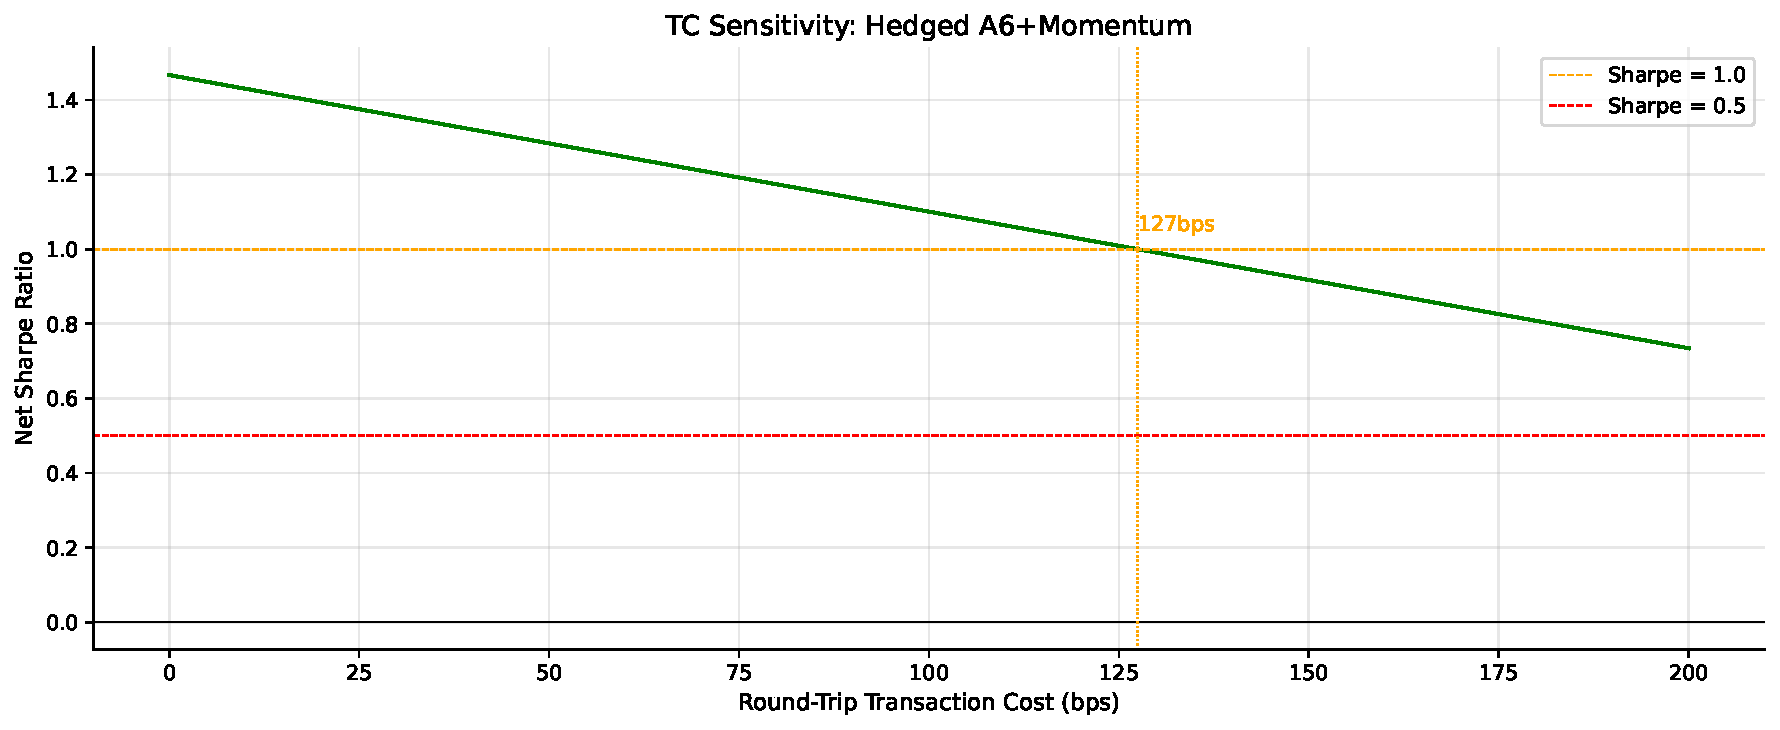
\includegraphics[width=0.85\textwidth]{nb09_tc_sensitivity.pdf}
    \caption{Transaction cost sensitivity: net Sharpe ratio of the hedged A6+Momentum strategy as a function of round-trip transaction costs (bps). Horizontal lines indicate Sharpe $= 1.0$ and Sharpe $= 0.5$ thresholds. The break-even for Sharpe $> 1.0$ is 127 bps.}
    \label{fig:tc}
\end{figure}

Under the country-weighted TC model (Section~\ref{sec:method}), the portfolio-weighted average cost is 44.6 bps, yielding a net hedged Sharpe of 1.303---comfortably above 1.0. Figure~\ref{fig:country_tc} illustrates the cross-country dispersion of TC estimates and the portfolio-weighted average over time. The break-even TC of 127 bps provides a 2.8$\times$ safety margin over the country-weighted average, confirming implementability even under conservative cost assumptions.

\begin{figure}[H]
    \centering
    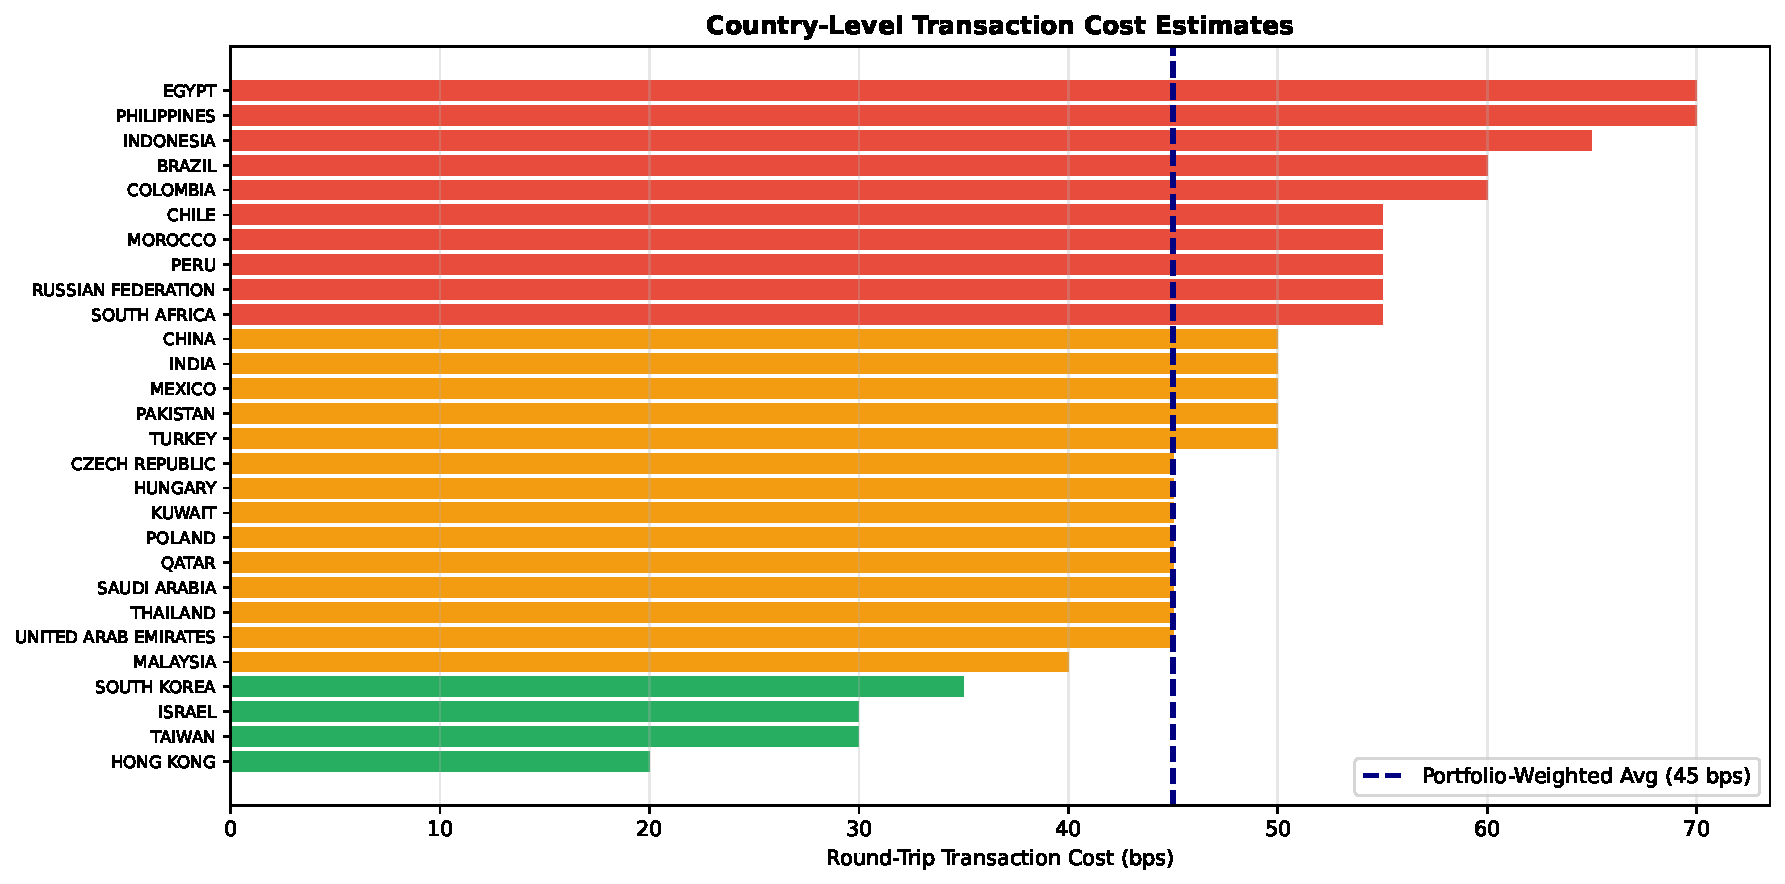
\includegraphics[width=0.85\textwidth]{country_tc_estimates.pdf}
    \caption{Country-level transaction cost estimates (bps) and the time-varying portfolio-weighted average TC. The dashed line indicates the overall average of 44.6 bps.}
    \label{fig:country_tc}
\end{figure}


% ==================================================================
% 6. PERFORMANCE ATTRIBUTION
% ==================================================================
\section{Performance Attribution}
\label{sec:attribution}

\subsection{Industry-Level Attribution}

The eleven industry factor portfolios exhibit moderate cross-correlation (average pairwise $\rho = 0.573$, range 0.393--0.778), providing genuine diversification benefits when combined. Table~\ref{tab:industry_perf} reports per-industry performance and return contribution to the final A6+Momentum portfolio.

\begin{table}[H]
\centering
\caption{Per-Industry Performance and Return Contribution}
\label{tab:industry_perf}
\small
\begin{tabular}{lccccc}
\toprule
\textbf{Industry} & \textbf{Sharpe} & \textbf{Ann.\ Ret} & \textbf{Ann.\ Vol} & \textbf{Avg Weight} & \textbf{Contribution} \\
\midrule
TECNO & 0.813 & 18.6\% & 22.9\% & 12.4\% & 24.3\% \\
TELCM & 0.647 & 11.9\% & 18.4\% & 8.3\%  & 14.3\% \\
FINAN & 0.541 & 10.7\% & 19.7\% & 8.4\%  & 2.3\% \\
CODIS & 0.530 & 11.9\% & 22.4\% & 8.3\%  & 2.3\% \\
UTILS & 0.520 & 11.4\% & 21.9\% & 10.1\% & 8.4\% \\
HLTHC & 0.468 & 10.9\% & 23.2\% & 8.3\%  & 5.2\% \\
COSTP & 0.463 &  7.9\% & 17.1\% & 6.8\%  & 5.5\% \\
ENEGY & 0.452 & 10.5\% & 23.2\% & 10.2\% & 12.4\% \\
BMATR & 0.397 & 10.2\% & 25.8\% & 9.0\%  & 12.6\% \\
INDUS & 0.384 &  8.8\% & 22.9\% & 8.6\%  & 6.6\% \\
RLEST & 0.337 & 10.6\% & 31.4\% & 9.6\%  & 6.0\% \\
\bottomrule
\end{tabular}
\begin{minipage}{\textwidth}
\vspace{0.3em}
\footnotesize
\textit{Notes:} Contribution is the fraction of total cumulative return attributable to each industry ($w_i \times r_i$ summed over time, as a percentage of total). Avg Weight reflects the time-average momentum weight. TECNO receives the highest average weight (12.4\% vs.\ EW 9.1\%) due to strong trailing returns, and contributes 24.3\% of total portfolio return.
\end{minipage}
\end{table}

\begin{figure}[H]
    \centering
    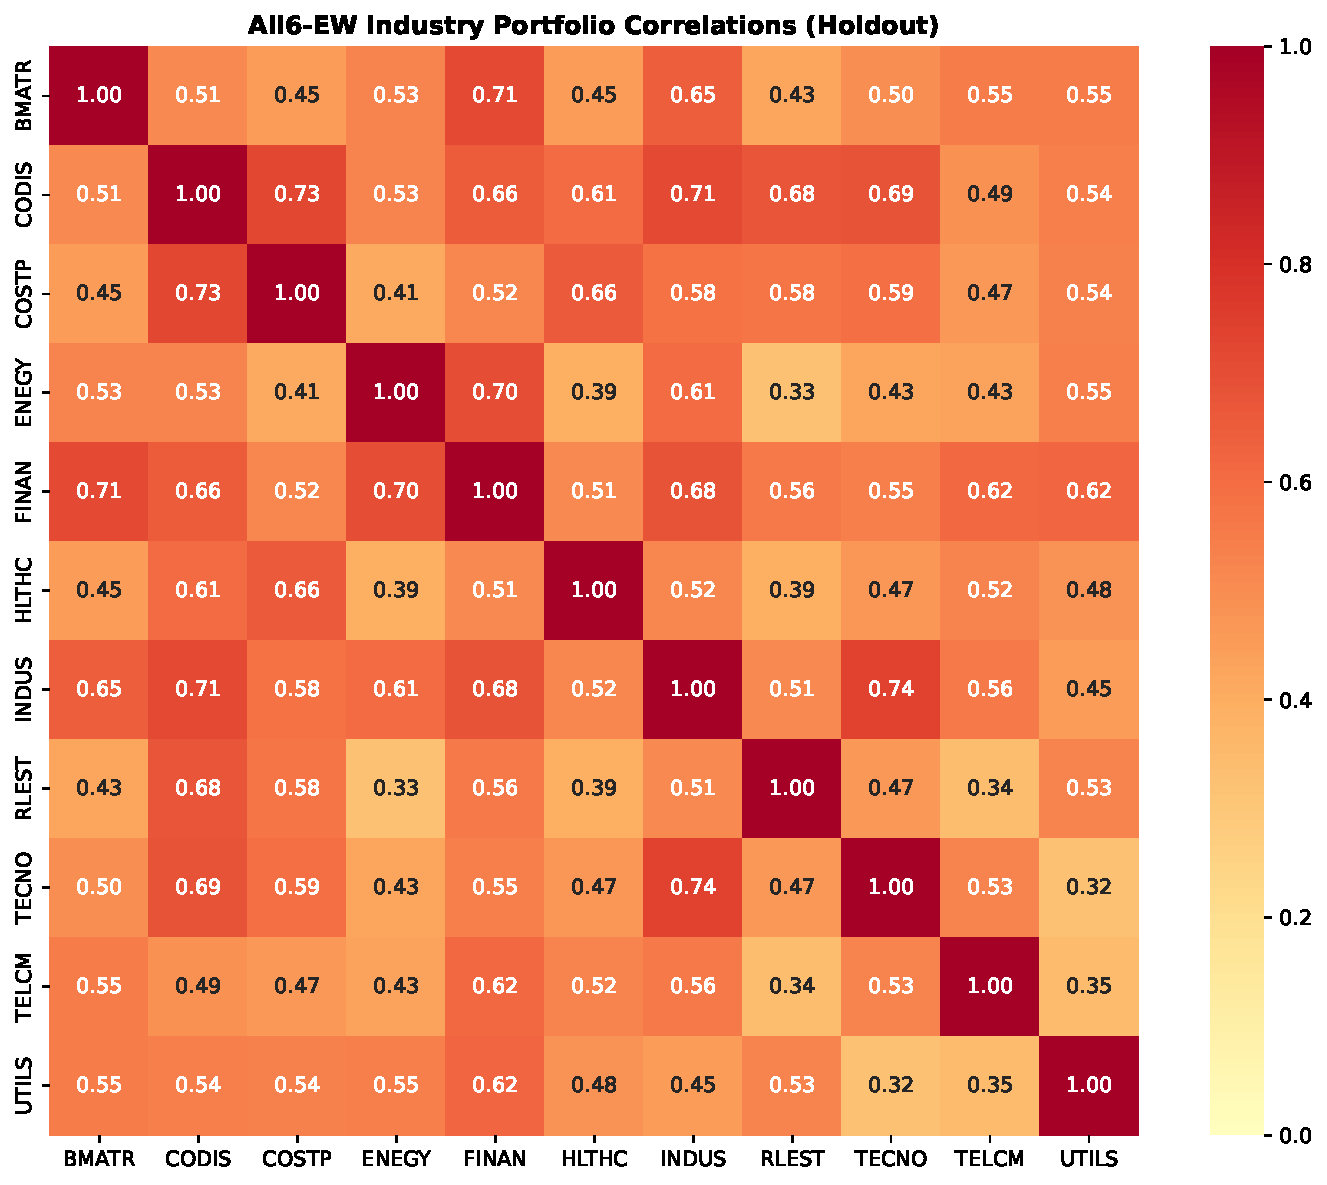
\includegraphics[width=0.85\textwidth]{nb08_industry_corr.pdf}
    \caption{Correlation heatmap of the eleven All6-EW industry factor portfolios. Average pairwise correlation is 0.573, indicating moderate diversification across industries.}
    \label{fig:industry_corr}
\end{figure}

\subsection{Momentum Weight Mechanics}

The momentum-weighted allocation dynamically shifts portfolio exposure toward industries with stronger trailing 12-month performance. Figure~\ref{fig:weights} illustrates the weight evolution over time.

\begin{figure}[H]
    \centering
    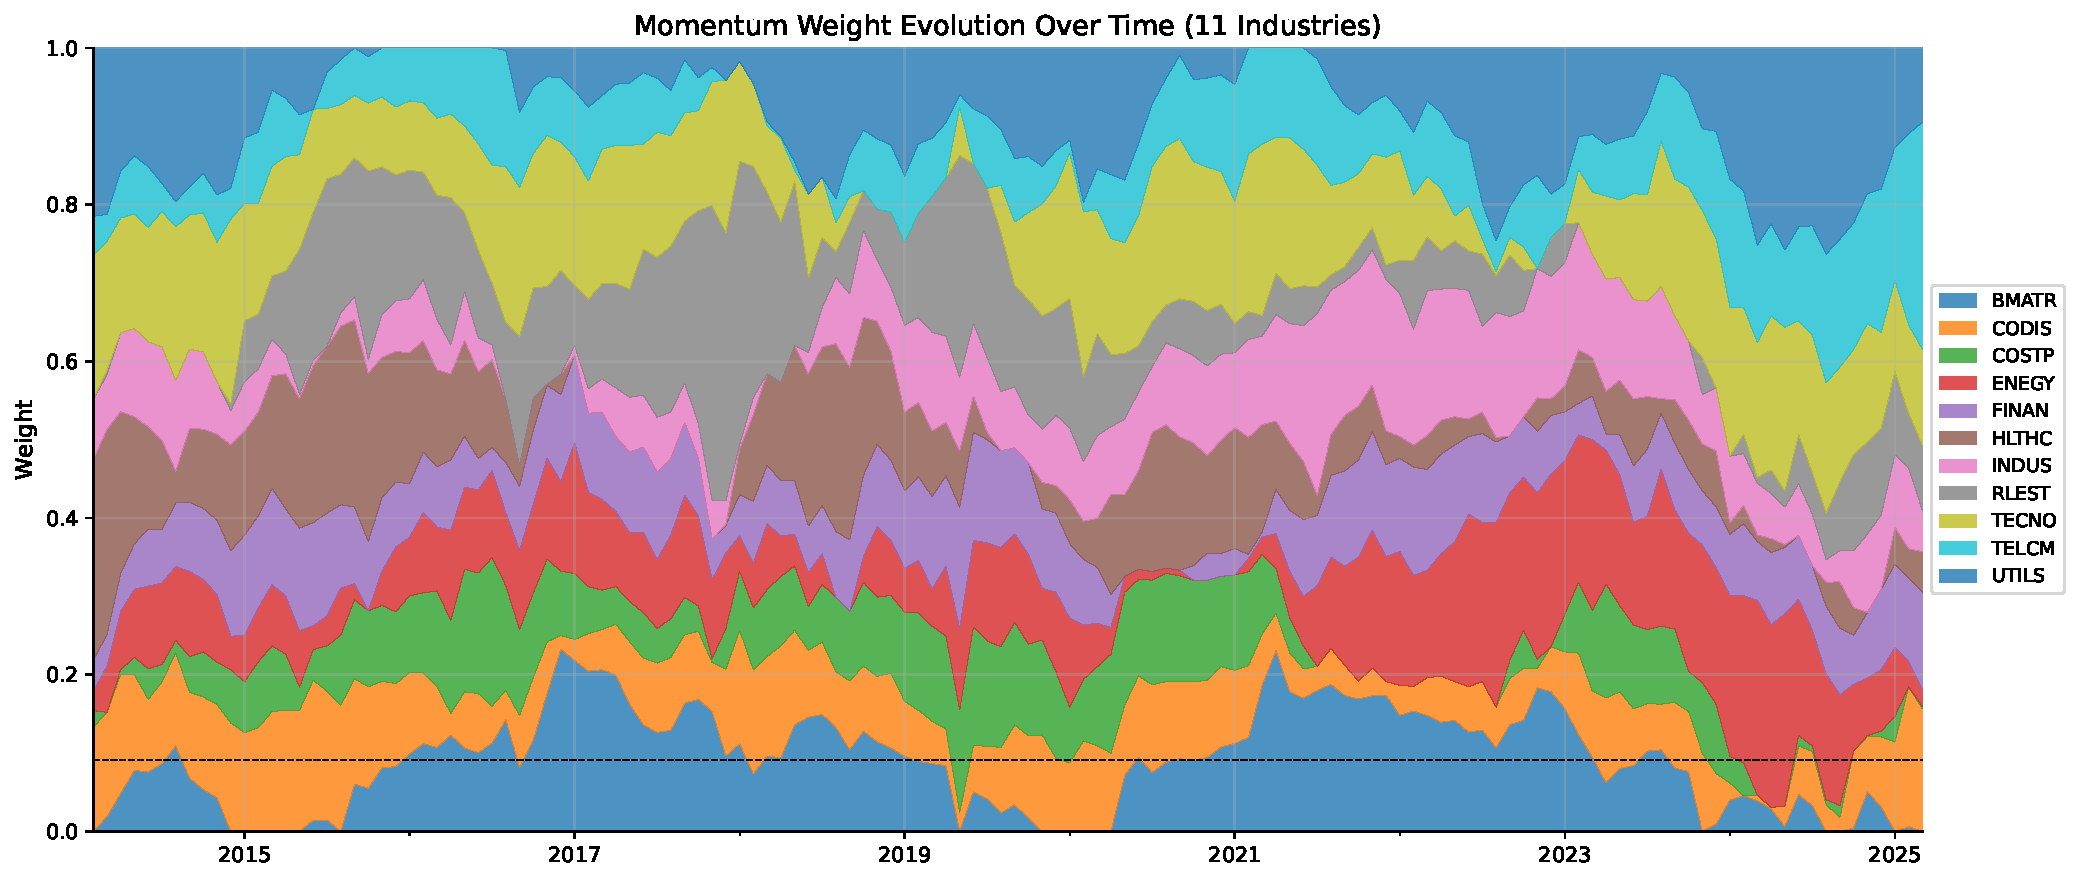
\includegraphics[width=0.95\textwidth]{nb08_weight_evolution.pdf}
    \caption{Momentum weight evolution across 11 industries (2014--2025). Industries with higher trailing 12-month returns receive proportionally more weight, subject to the floor that ensures all industries retain some allocation.}
    \label{fig:weights}
\end{figure}

Weight concentration, measured by the Herfindahl-Hirschman Index (HHI), averages 0.131 (vs.\ 0.091 for equal weighting), indicating moderate concentration. No single industry ever exceeds approximately 20\% weight, preventing excessive sector bets.

\subsection{Alpha Stability}

Table~\ref{tab:annual_alpha} presents the annual decomposition of hedged alpha. Alpha is positive in every year of the sample, ranging from 3.9\% (2019) to 16.9\% (2020). The annualized Sharpe ratio exceeds 0.9 in every year, demonstrating the consistency of the alpha stream.

\begin{table}[H]
\centering
\caption{Annual Alpha Decomposition (Hedged A6+Momentum)}
\label{tab:annual_alpha}
\small
\begin{tabular}{lccccc}
\toprule
\textbf{Year} & \textbf{Alpha (ann.)} & \textbf{Vol} & \textbf{Sharpe} & \textbf{Hit Rate} & \textbf{Months} \\
\midrule
2019 &  3.9\% & 4.3\% & 0.91 & 64\% & 11 \\
2020 & 16.9\% & 6.3\% & 2.68 & 75\% & 12 \\
2021 & 10.1\% & 7.0\% & 1.43 & 67\% & 12 \\
2022 &  9.3\% & 7.2\% & 1.30 & 58\% & 12 \\
2023 &  8.6\% & 7.1\% & 1.22 & 58\% & 12 \\
2024 &  4.9\% & 5.0\% & 0.97 & 50\% & 12 \\
2025 &  5.4\% & 0.7\% & 8.13 & 100\% & 3 \\
\bottomrule
\end{tabular}
\begin{minipage}{\textwidth}
\vspace{0.3em}
\footnotesize
\textit{Notes:} 2025 data covers only January--March. Alpha is positive in every full year. The 2020 spike reflects strong factor performance during the COVID-19 recovery, when momentum and low-volatility stocks substantially outperformed.
\end{minipage}
\end{table}

\begin{figure}[H]
    \centering
    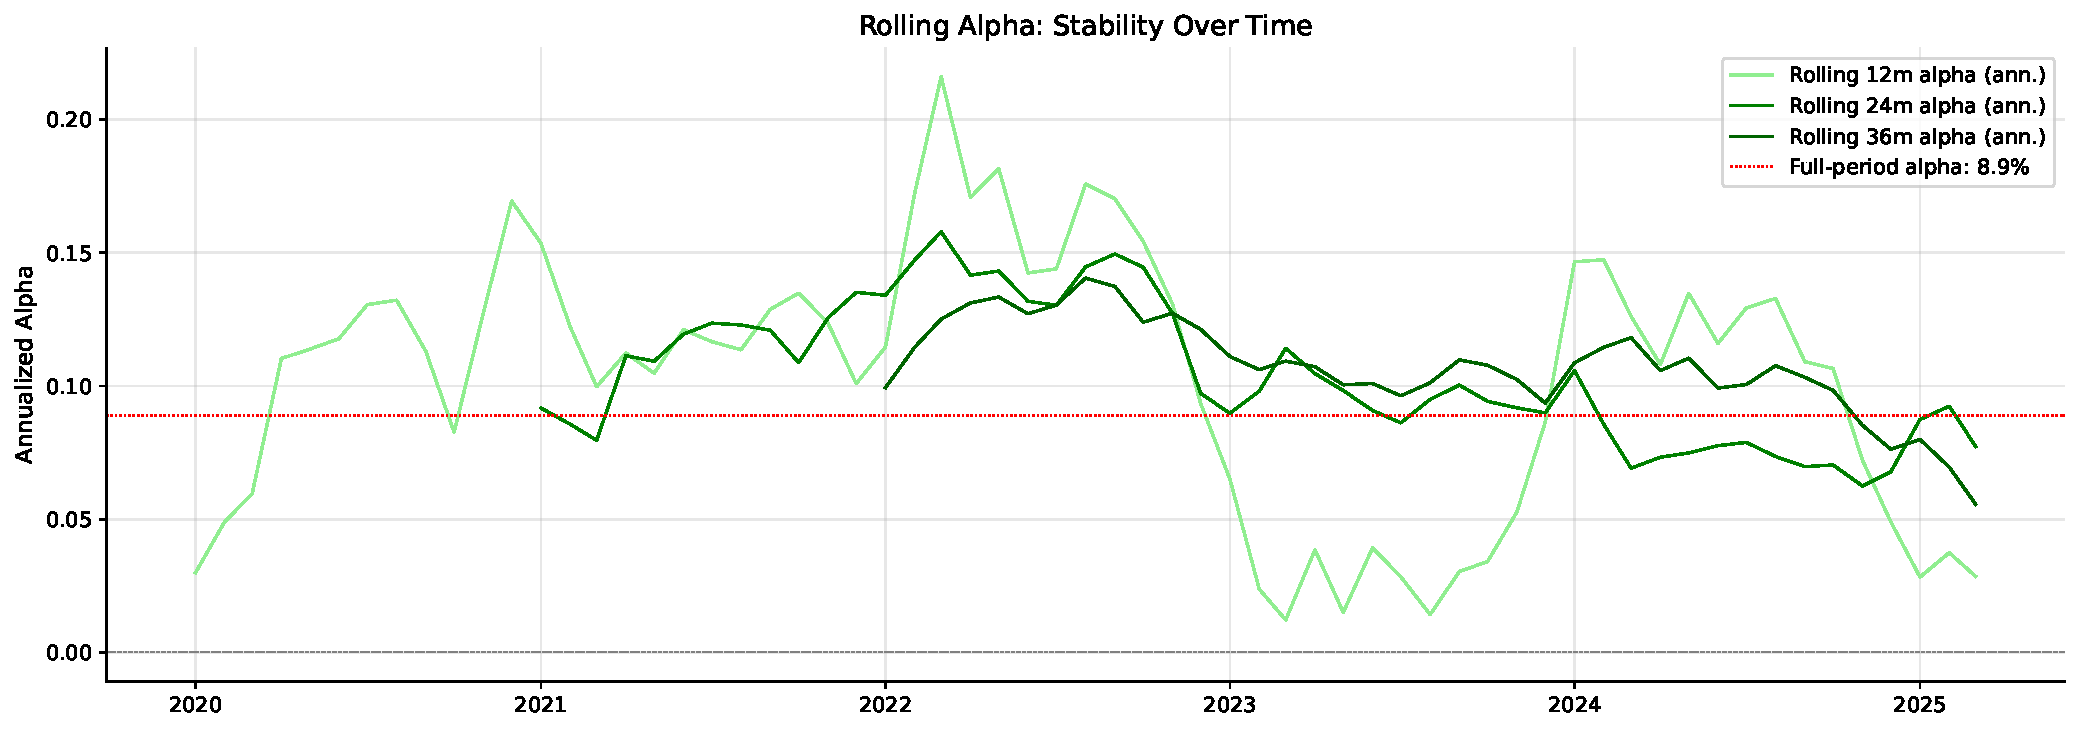
\includegraphics[width=0.85\textwidth]{nb09_rolling_alpha.pdf}
    \caption{Rolling 12-month, 24-month, and 36-month annualized alpha (hedged A6+Momentum). The red dotted line shows the full-period alpha of 8.9\%. Rolling alpha remains positive in nearly all periods.}
    \label{fig:rolling_alpha}
\end{figure}

\subsection{Regime Analysis}

A critical test of any hedged strategy is whether it generates alpha in both rising and falling market environments. Table~\ref{tab:regime} splits the hedged sample into months where the MSCI EM benchmark return was positive (``EM Up'') versus negative (``EM Down'').

\begin{table}[H]
\centering
\caption{Performance by Market Regime}
\label{tab:regime}
\small
\begin{tabular}{lccc}
\toprule
\textbf{Metric} & \textbf{EM Up (41 months)} & \textbf{EM Down (33 months)} & \textbf{All (74 months)} \\
\midrule
Hedged mean (monthly)      & $+$0.94\% & $+$0.49\% & $+$0.74\% \\
Hedged hit rate             & 68\%      & 58\%      & 64\% \\
Unhedged mean (monthly)     & $+$4.16\% & $-$3.11\% & $+$0.92\% \\
Benchmark mean (monthly)    & $+$3.63\% & $-$4.03\% & $+$0.22\% \\
\bottomrule
\end{tabular}
\begin{minipage}{\textwidth}
\vspace{0.3em}
\footnotesize
\textit{Notes:} The hedged strategy generates positive alpha in \emph{both} up and down EM markets, confirming that the alpha is not simply a leveraged market bet. The correlation between hedged returns and the MSCI EM benchmark is 0.07 (near zero), indicating effective market neutrality.
\end{minipage}
\end{table}

\subsection{Volatility Decomposition}

The unhedged portfolio's total volatility (17.1\% annualized) decomposes into systematic and idiosyncratic components:

\begin{itemize}
    \item \textbf{Systematic} ($\beta \times \sigma_{\text{EM}}$): $0.893 \times 17.5\% = 15.6\%$ (92\% of total variance)
    \item \textbf{Idiosyncratic}: $\sqrt{17.1\%^2 - 15.6\%^2} = 6.8\%$ (40\% of total vol, but only 8\% of variance)
    \item \textbf{Hedged vol (actual)}: 6.1\%
\end{itemize}

The hedge removes the dominant systematic component, leaving only the idiosyncratic alpha stream. The actual hedged volatility (6.1\%) is slightly lower than the theoretical idiosyncratic component (6.8\%), reflecting the time-varying nature of beta that provides additional diversification.

\begin{figure}[H]
    \centering
    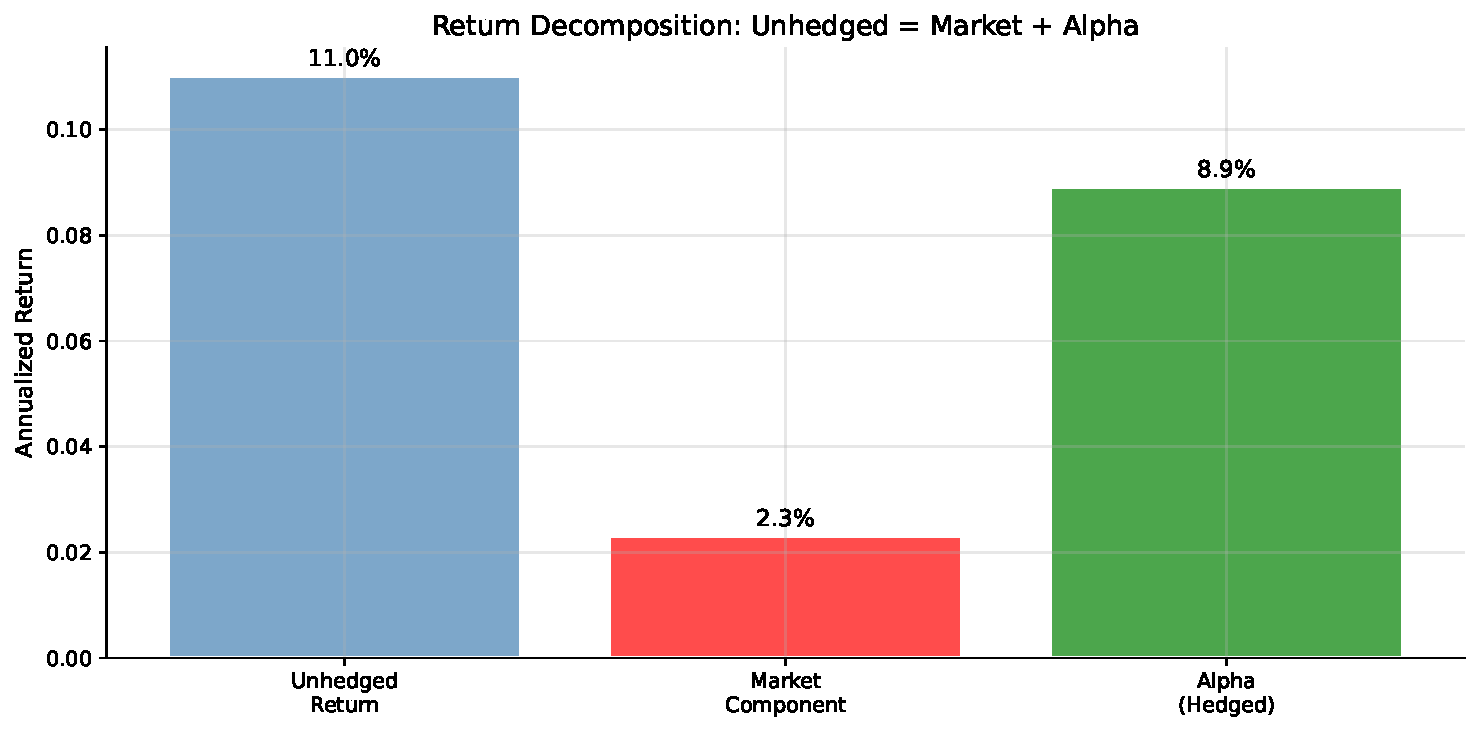
\includegraphics[width=0.75\textwidth]{nb09_return_waterfall.pdf}
    \caption{Return decomposition: the unhedged annual return equals the market component ($\beta \times$ benchmark return) plus alpha. Hedging removes the market component, isolating the alpha.}
    \label{fig:waterfall}
\end{figure}

\subsection{Drawdown Analysis}

Hedging dramatically reduces drawdown risk. The maximum drawdown of the hedged strategy is 7.2\%, compared to 24.0\% for the unhedged strategy and 38.4\% for the MSCI EM Index over the same period.

\begin{figure}[H]
    \centering
    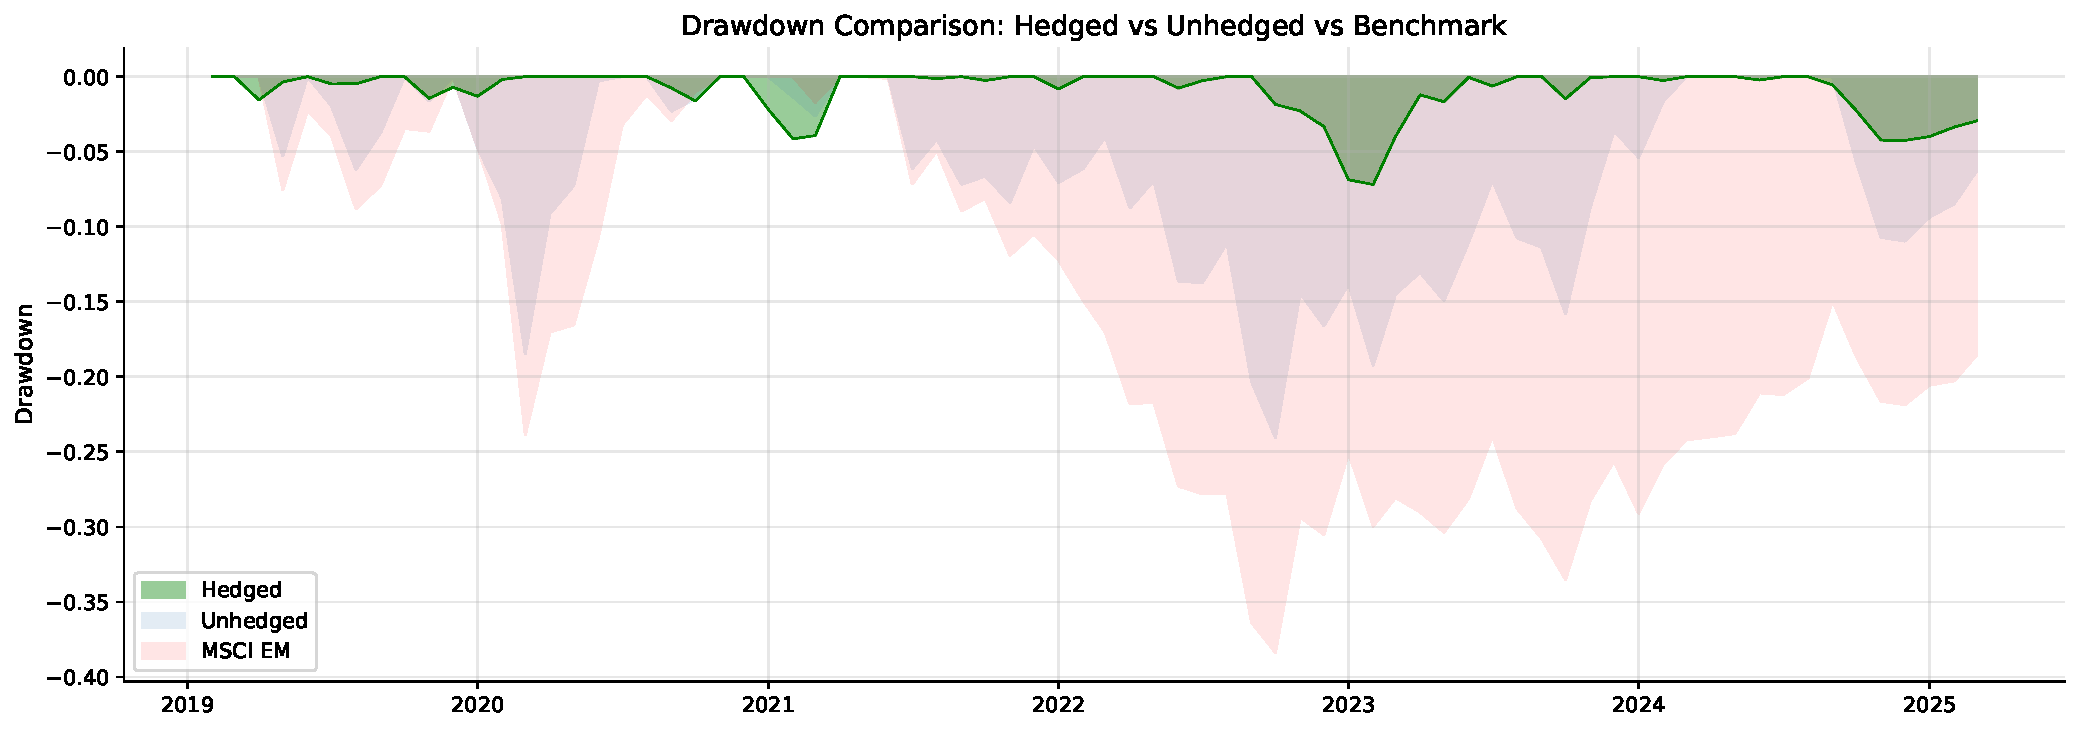
\includegraphics[width=0.85\textwidth]{nb09_drawdown.pdf}
    \caption{Drawdown comparison: hedged (green), unhedged (blue), and MSCI EM (red). The hedge reduces maximum drawdown by a factor of 3.4$\times$ relative to the unhedged portfolio and 5.3$\times$ relative to the benchmark.}
    \label{fig:drawdown}
\end{figure}

\subsection{Return Distribution}

The hedged return distribution exhibits favorable properties relative to the unhedged distribution:

\begin{itemize}
    \item \textbf{Positive skewness}: 0.24 (hedged) vs.\ 0.06 (unhedged) vs.\ $-$0.03 (MSCI EM)
    \item \textbf{Low kurtosis}: $-$0.04 (hedged), indicating near-normal tails
    \item \textbf{Tighter extremes}: worst month $-$3.7\% (hedged) vs.\ $-$11.3\% (unhedged) vs.\ $-$15.6\% (MSCI EM)
    \item \textbf{Higher hit rate}: 63.5\% (hedged) vs.\ 59.5\% (unhedged) vs.\ 55.4\% (MSCI EM)
\end{itemize}


% ==================================================================
% 7. ROBUSTNESS
% ==================================================================
\section{Robustness and Sensitivity Analysis}
\label{sec:robustness}

\subsection{In-Sample vs.\ Out-of-Sample Stability}

All strategies exhibit IS-to-OOS degradation, which is expected in any backtest. The key metric is the degree of degradation and whether OOS performance remains economically meaningful. Table~\ref{tab:is_oos} shows that All6-EW has the most favorable OOS retention:

\begin{table}[H]
\centering
\caption{IS vs.\ OOS Sharpe Ratio}
\label{tab:is_oos}
\small
\begin{tabular}{lccc}
\toprule
\textbf{Variant} & \textbf{IS Sharpe} & \textbf{OOS Sharpe} & \textbf{Retention} \\
\midrule
All6-EW     & 0.979 & 0.444 & 45\% \\
SF (best-1) & 0.930 & 0.414 & 45\% \\
Top3-EW     & 0.997 & 0.382 & 38\% \\
Corr03-EW   & 1.013 & 0.369 & 36\% \\
MSCI EM     & 0.689 & 0.142 & 21\% \\
\bottomrule
\end{tabular}
\begin{minipage}{\textwidth}
\vspace{0.3em}
\footnotesize
\textit{Notes:} Retention = OOS Sharpe / IS Sharpe. All6-EW has the highest retention rate among the composite strategies, consistent with its avoidance of estimation error.
\end{minipage}
\end{table}

\subsection{Covariance Estimator Sensitivity}

We test three covariance estimation approaches for portfolio construction: Ledoit-Wolf shrinkage (baseline), sample covariance, and exponentially-weighted moving average (EWMA). The results show that Momentum and EqualWeight are completely insensitive to the covariance choice (as expected, since Momentum does not use the covariance matrix and EqualWeight ignores it by construction). TO\_MVO and Black-Litterman show moderate sensitivity, with Ledoit-Wolf and sample covariance performing similarly and EWMA slightly worse.

\subsection{Estimation Window Length}

We compare 36-month and 60-month rolling windows for both IC estimation and covariance estimation. Results are robust, with 60-month windows generally producing slightly higher Sharpe ratios. The exception is MeanCVaR, which performs better with 36-month windows, and HRP, which shows mixed results.

\subsection{Country-Weighted Transaction Cost Robustness}

As a robustness check on the implementability of our strategy, we replace the uniform 20 bps TC assumption with country-specific estimates averaging 44.6 bps (Table~\ref{tab:country_tc}). This more than doubles the cost drag relative to the baseline. Table~\ref{tab:hedged} reports the impact: A6+Momentum's hedged Sharpe declines from 1.393 (at 20 bps) to 1.303 (at 45 bps), a reduction of 6.5\%. The strategy remains the only one to exceed Sharpe 1.0 under both cost assumptions, confirming its robustness to realistic EM implementation costs.

The difference between uniform and country-weighted costs is economically meaningful---approximately 90 basis points of annualized alpha drag---but does not alter any of the strategy rankings or main conclusions. The All6-EW factor composition continues to dominate all variants at the higher cost level (Table~\ref{tab:mf_tc}), and momentum-weighted portfolio construction remains the best allocation method.

\subsection{Look-Ahead Bias Audit}

We conducted a comprehensive, step-by-step audit of the entire pipeline to verify the absence of look-ahead bias:

\begin{enumerate}
    \item \textbf{Data processing}: Winsorization, neutralization, and imputation all use only cross-sectional data at month $t$, with no forward-looking information.

    \item \textbf{Factor selection}: Rolling IC uses only data from months $[t-60, t-1]$. The 20\% stability filter prevents excessive switching but does not introduce any future information.

    \item \textbf{Stock selection}: Factors at month $t$ predict returns at month $t+1$. The composite score uses only rolling ICs from the estimation window.

    \item \textbf{Portfolio construction}: Covariance and expected return estimates use only returns from $[t-60, t-1]$. Weight optimization occurs before month $t$ returns are realized.

    \item \textbf{Beta hedging}: $\hat{\beta}_t$ is estimated from $[t-60, t-1]$, excluding month $t$. The hedged return uses $\hat{\beta}_t \times r_{m,t}$, where $r_{m,t}$ is realized simultaneously with $r_{p,t}$ (contemporaneous hedging, which is implementable in practice).

    \item \textbf{IC measurement}: The IC correlates factor at $t$ with return at $t$ (contemporaneous), but the backtest uses factor at $t$ to trade at $t+1$. This means the IC may slightly overstate true predictive power, a standard feature of IC-based approaches that should be noted but does not constitute look-ahead bias.
\end{enumerate}

\subsection{Weight Concentration}

The Herfindahl-Hirschman Index (HHI) of momentum weights averages 0.131 (vs.\ 0.091 for equal weighting). The maximum HHI observed is 0.211, corresponding to a month where the top industry received approximately 20\% weight. This moderate concentration indicates that momentum weighting does not take extreme sector bets.


% ==================================================================
% 8. CONCLUSION
% ==================================================================
\section{Conclusion}
\label{sec:conclusion}

This paper presents a comprehensive investigation of factor investing in emerging markets, tracing the full pipeline from raw data through factor construction, multi-factor composition, cross-industry portfolio construction, and dynamic beta hedging.

Our principal findings are:

\begin{enumerate}
    \item \textbf{All six factors contain predictive information.} Size and value (P/B) exhibit the strongest rank ICs, while momentum, volatility, dividend yield, and quality also contribute cross-sectional predictive power across the eleven EM industry groups.

    \item \textbf{Simple factor combination dominates sophisticated alternatives.} Equal-weighting all six factors (All6-EW) achieves the highest out-of-sample Sharpe ratio (0.444), outperforming IC-weighted composites, IC-correlation-filtered variants, and Ridge/ElasticNet regression. This finding is consistent with the broad conclusion of \citet{demiguel2009} that estimation error makes naive diversification preferable to optimization in finite samples.

    \item \textbf{Momentum-weighted allocation is the best portfolio construction technique.} Among ten methods tested---including minimum variance, maximum Sharpe, risk parity, HRP, Black-Litterman, mean-CVaR, and turnover-penalized MVO---momentum-weighted allocation delivers the highest Sharpe ratio (0.594) by dynamically tilting toward outperforming sectors.

    \item \textbf{Dynamic beta hedging transforms the strategy.} Hedging the portfolio's rolling 60-month beta to the MSCI EM Index converts a moderate long-only strategy (Sharpe 0.59, vol 15.9\%) into a high-alpha market-neutral strategy (Sharpe 1.47, alpha 8.9\%, vol 6.1\%, max DD 7.2\%). Alpha is positive in both rising and falling EM markets, with a hedged-benchmark correlation of 0.07.

    \item \textbf{Results are robust to realistic implementation costs.} Under a country-weighted TC estimate of 44.6 bps---based on \citet{domowitz2001} and more than double the commonly assumed 20 bps---the hedged Sharpe remains 1.30. The break-even TC for Sharpe $> 1.0$ is 127 bps, providing a 2.8$\times$ safety margin over the country-weighted average. Results are also insensitive to covariance estimation method, estimation window length, and market regime. A comprehensive look-ahead bias audit confirms that no future information leaks into any stage of the pipeline.
\end{enumerate}

\paragraph{Limitations.} Our analysis is subject to several caveats. First, the strategy is backtested, not live-traded; implementation slippage and market impact may reduce realized returns, particularly for less liquid EM stocks. Second, survivorship bias may be present in the MSCI EM Index constituents, though the annual reconstitution mitigates this concern. Third, we use a single benchmark (MSCI EM) for hedging; alternative hedges (e.g., EM ETFs, futures) may have different implementation characteristics. Fourth, the hedged sample (74 months, 2019--2025) is relatively short, and the alpha may partially reflect favorable market conditions for factor strategies during this period.

\paragraph{Future work.} Several extensions are natural. First, country-level factor models could capture additional cross-sectional variation. Second, dynamic factor timing---adjusting factor weights based on macro conditions---could improve alpha stability. Third, incorporating alternative hedge instruments (EM futures, sector ETFs) may reduce hedging costs and improve implementability for institutional investors.


% ==================================================================
% REFERENCES
% ==================================================================
\newpage
\bibliographystyle{plainnat}
\bibliography{references}


% ==================================================================
% APPENDIX
% ==================================================================
\newpage
\appendix
\section{Portfolio Construction Method Formulations}
\label{app:methods}

\subsection{Equal Weight}
\begin{equation}
    w_i = \frac{1}{N}, \quad i = 1, \ldots, N
\end{equation}

\subsection{Inverse Volatility}
\begin{equation}
    w_i = \frac{1/\sigma_i}{\sum_{j=1}^N 1/\sigma_j}
\end{equation}

\subsection{Minimum Variance}
\begin{equation}
    \min_{\mathbf{w}} \mathbf{w}'\boldsymbol{\Sigma}\mathbf{w} \quad \text{s.t.} \quad \mathbf{1}'\mathbf{w} = 1, \quad w_i \in [0.02, 0.20]
\end{equation}

\subsection{Maximum Sharpe Ratio}
\begin{equation}
    \max_{\mathbf{w}} \frac{\mathbf{w}'\boldsymbol{\mu}}{\sqrt{\mathbf{w}'\boldsymbol{\Sigma}\mathbf{w}}} \quad \text{s.t.} \quad \mathbf{1}'\mathbf{w} = 1, \quad w_i \in [0.02, 0.20]
\end{equation}

\subsection{Risk Parity}
\begin{equation}
    w_i \frac{\partial \sigma_p}{\partial w_i} = \frac{\sigma_p}{N}, \quad \forall i
\end{equation}

\subsection{Hierarchical Risk Parity}
Following \citet{lopezdeprado2016}: (i) cluster assets by correlation distance, (ii) quasi-diagonalize the covariance matrix, (iii) allocate using recursive bisection with inverse-variance weights within clusters.

\subsection{Momentum-Weighted}
\begin{equation}
    \tilde{w}_i = \bar{r}_i^{(12)} - \min_j \bar{r}_j^{(12)} + \epsilon, \quad w_i = \frac{\tilde{w}_i}{\sum_j \tilde{w}_j}
\end{equation}

\subsection{Black-Litterman}
\begin{equation}
    \boldsymbol{\mu}_{\text{BL}} = [(\tau\boldsymbol{\Sigma})^{-1} + \mathbf{P}'\boldsymbol{\Omega}^{-1}\mathbf{P}]^{-1}[(\tau\boldsymbol{\Sigma})^{-1}\boldsymbol{\pi} + \mathbf{P}'\boldsymbol{\Omega}^{-1}\mathbf{q}]
\end{equation}
where $\boldsymbol{\pi}$ is the equilibrium expected return and $(\mathbf{P}, \mathbf{q})$ encode IC-based views.

\subsection{Mean-CVaR}
\begin{equation}
    \min_{\mathbf{w}} \text{CVaR}_{0.95}(\mathbf{w}) \quad \text{s.t.} \quad \mathbf{1}'\mathbf{w} = 1, \quad w_i \in [0.02, 0.20]
\end{equation}

\subsection{Turnover-Penalized MVO}
\begin{equation}
    \max_{\mathbf{w}} \left[\mathbf{w}'\boldsymbol{\mu} - \frac{1}{2}\mathbf{w}'\boldsymbol{\Sigma}\mathbf{w} - \gamma \|\mathbf{w} - \mathbf{w}_{\text{prev}}\|_1\right] \quad \text{s.t.} \quad \mathbf{1}'\mathbf{w} = 1
\end{equation}
with $\gamma = 0.001$.


\section{Additional Figures}

\begin{figure}[H]
    \centering
    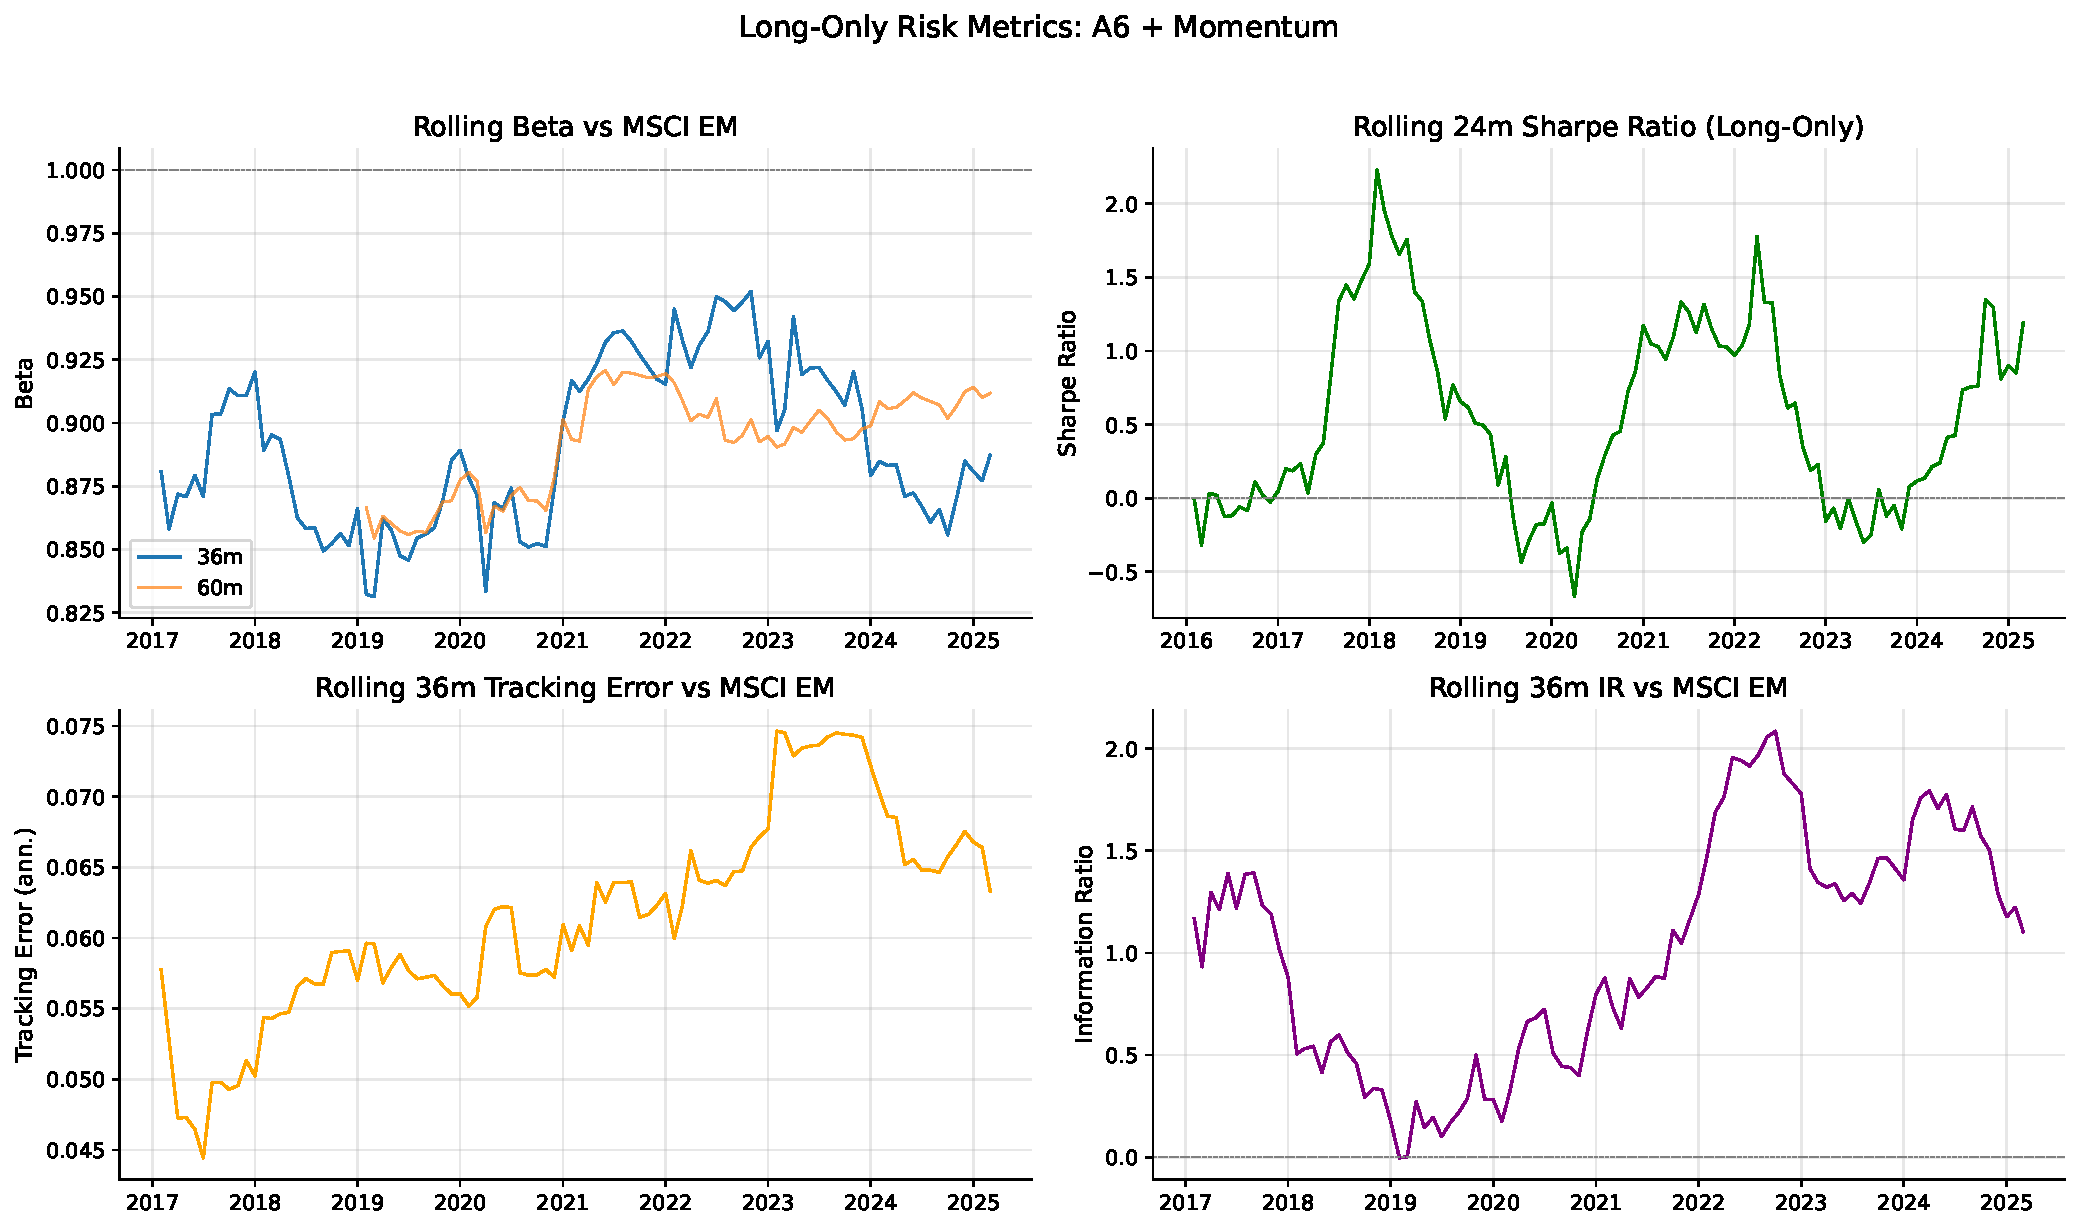
\includegraphics[width=0.85\textwidth]{nb08_rolling_risk.pdf}
    \caption{Rolling risk metrics for the long-only A6+Momentum strategy: (a) rolling 36m/60m beta vs.\ MSCI EM, (b) rolling 24m Sharpe ratio, (c) rolling 36m tracking error, (d) rolling 36m information ratio.}
    \label{fig:rolling_risk}
\end{figure}

\begin{figure}[H]
    \centering
    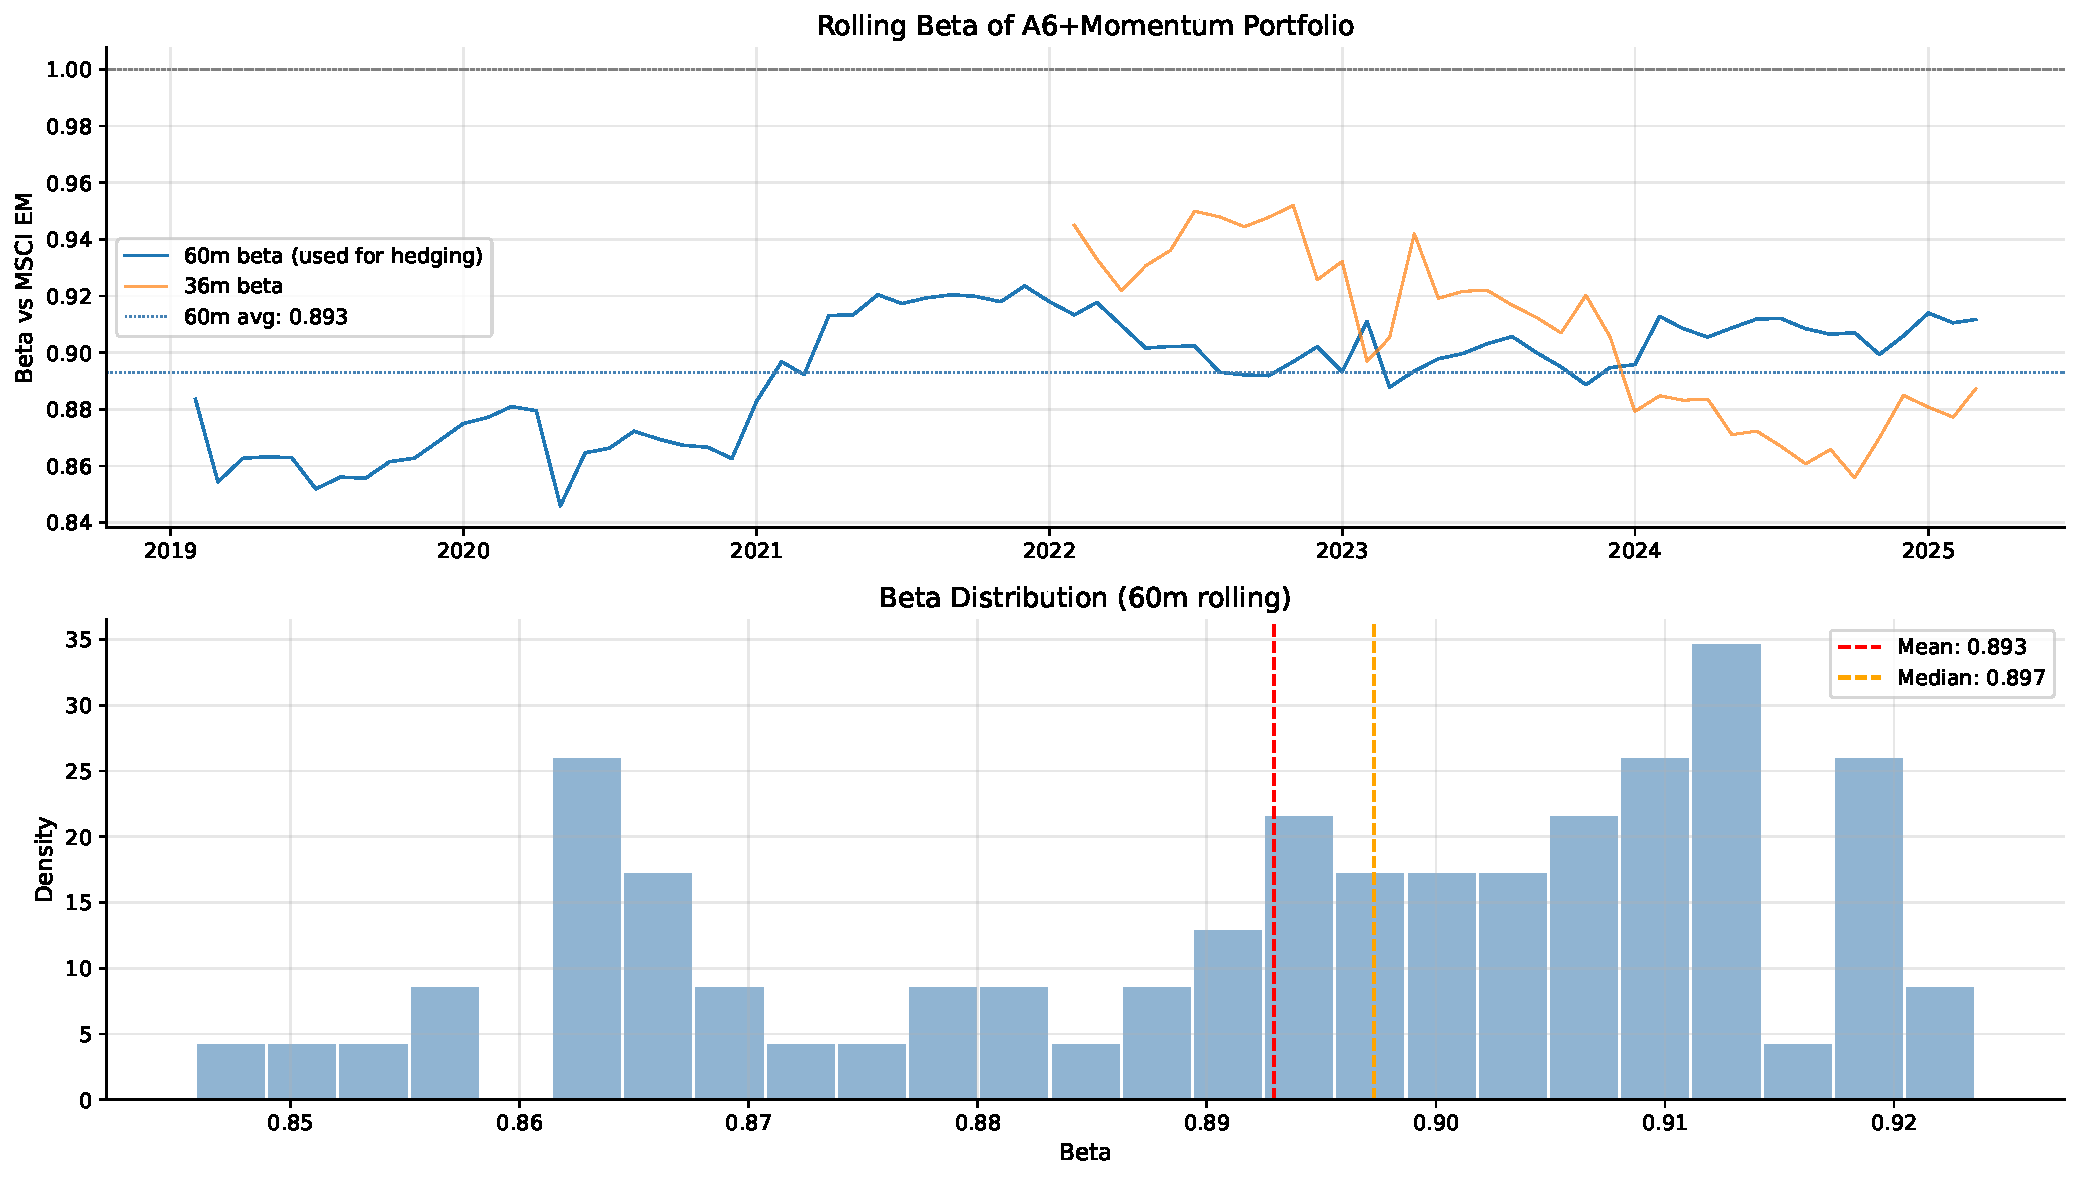
\includegraphics[width=0.85\textwidth]{nb09_beta_dynamics.pdf}
    \caption{Beta dynamics of the A6+Momentum portfolio: (top) rolling 60-month and 36-month beta time series, (bottom) histogram of beta values. Average beta is 0.893, with a standard deviation of 0.021.}
    \label{fig:beta}
\end{figure}

\begin{figure}[H]
    \centering
    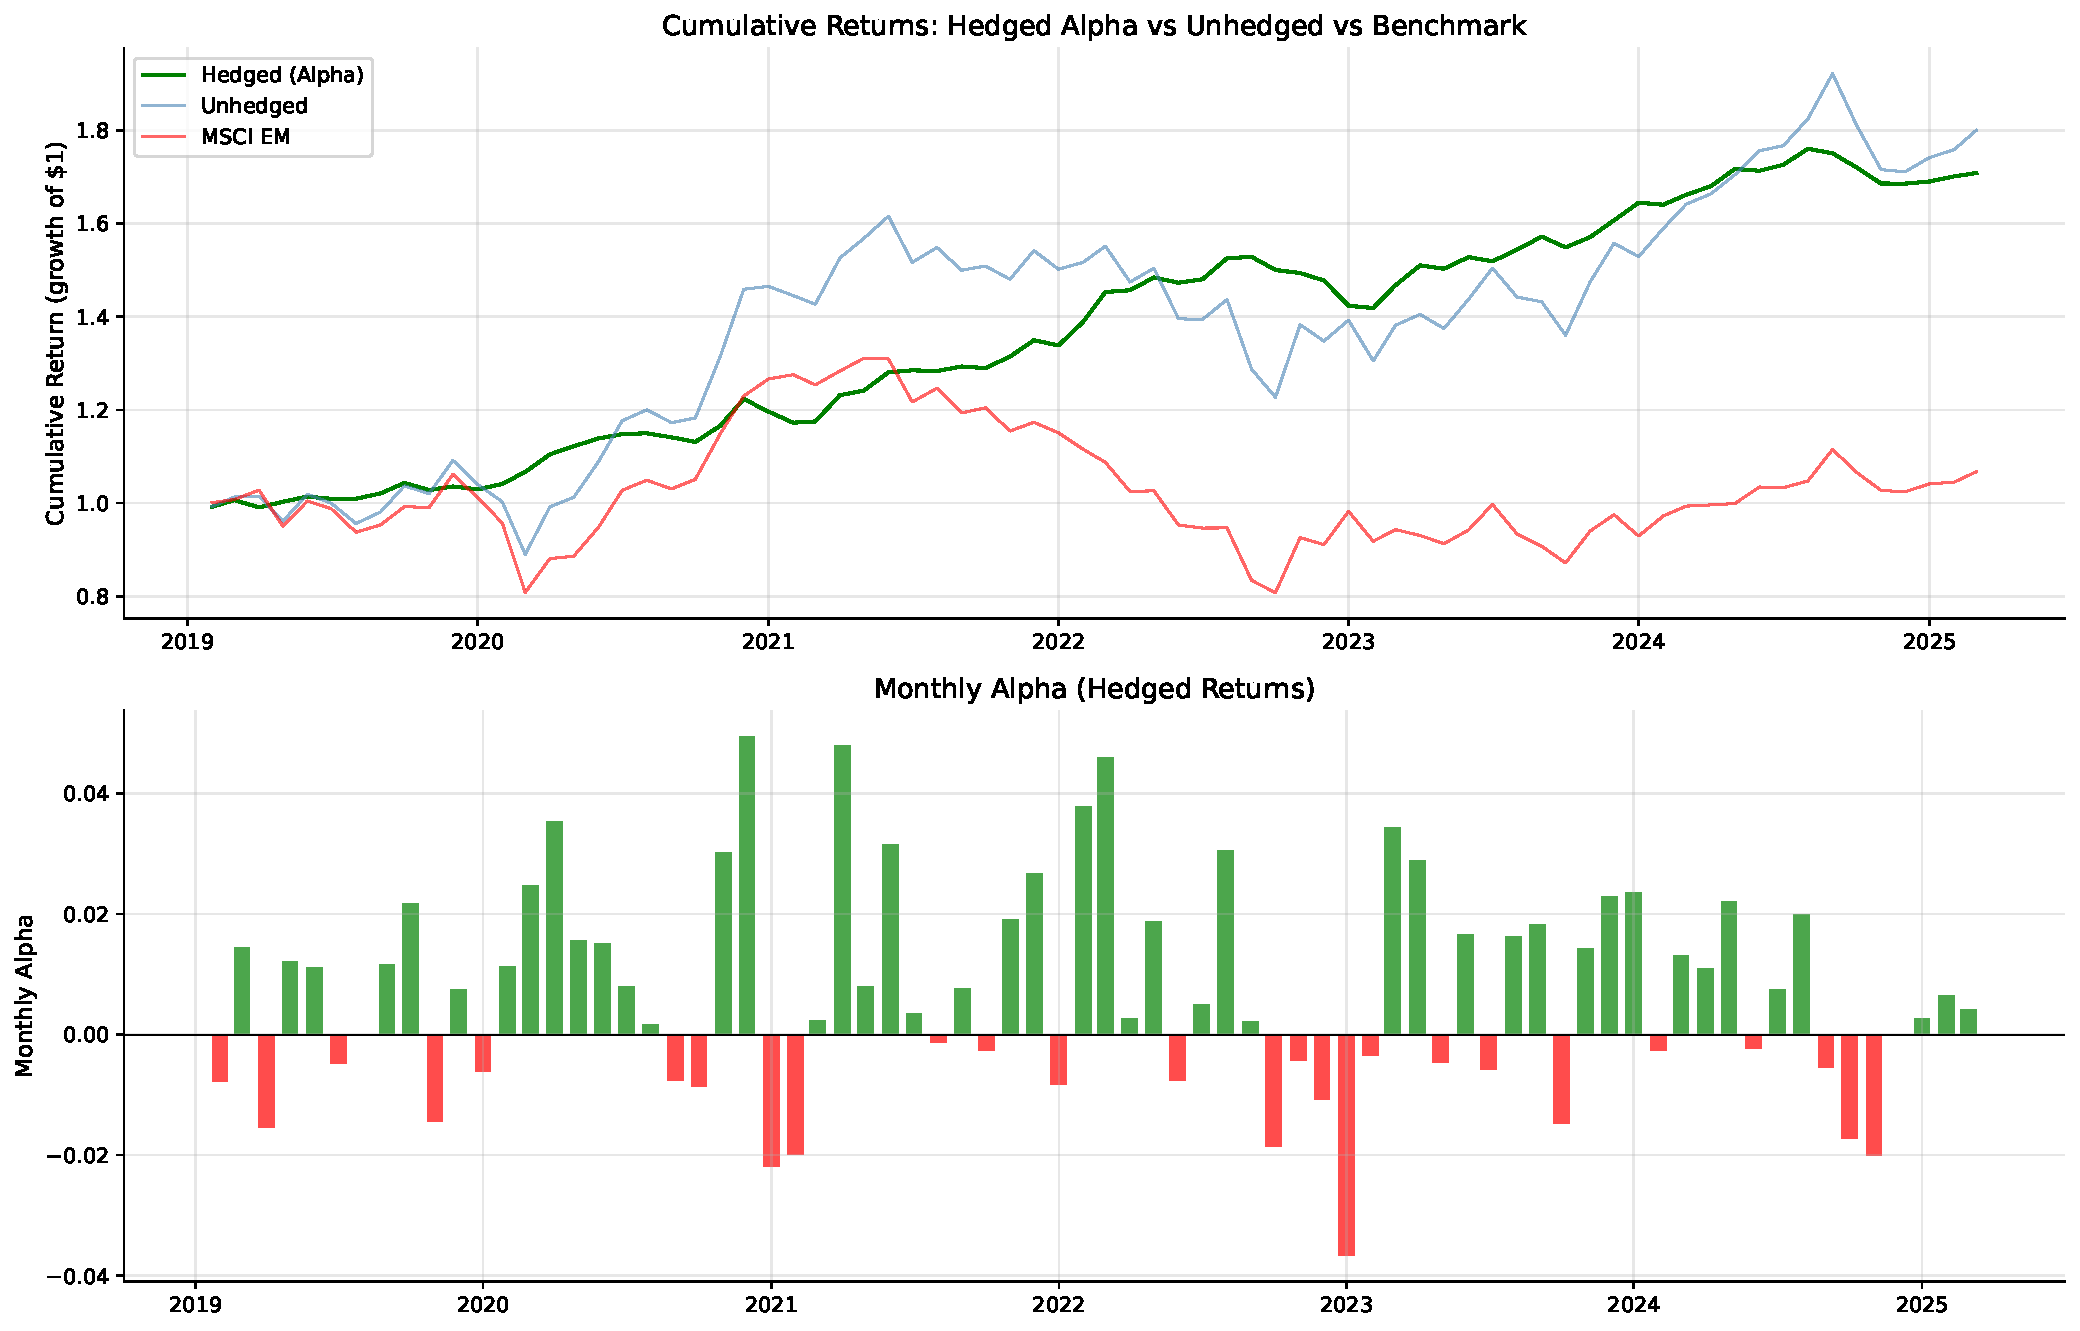
\includegraphics[width=0.85\textwidth]{nb09_alpha_timeseries.pdf}
    \caption{Alpha time series: (top) cumulative returns for hedged alpha, unhedged portfolio, and MSCI EM, (bottom) monthly hedged alpha (green = positive, red = negative).}
    \label{fig:alpha_ts}
\end{figure}

\begin{figure}[H]
    \centering
    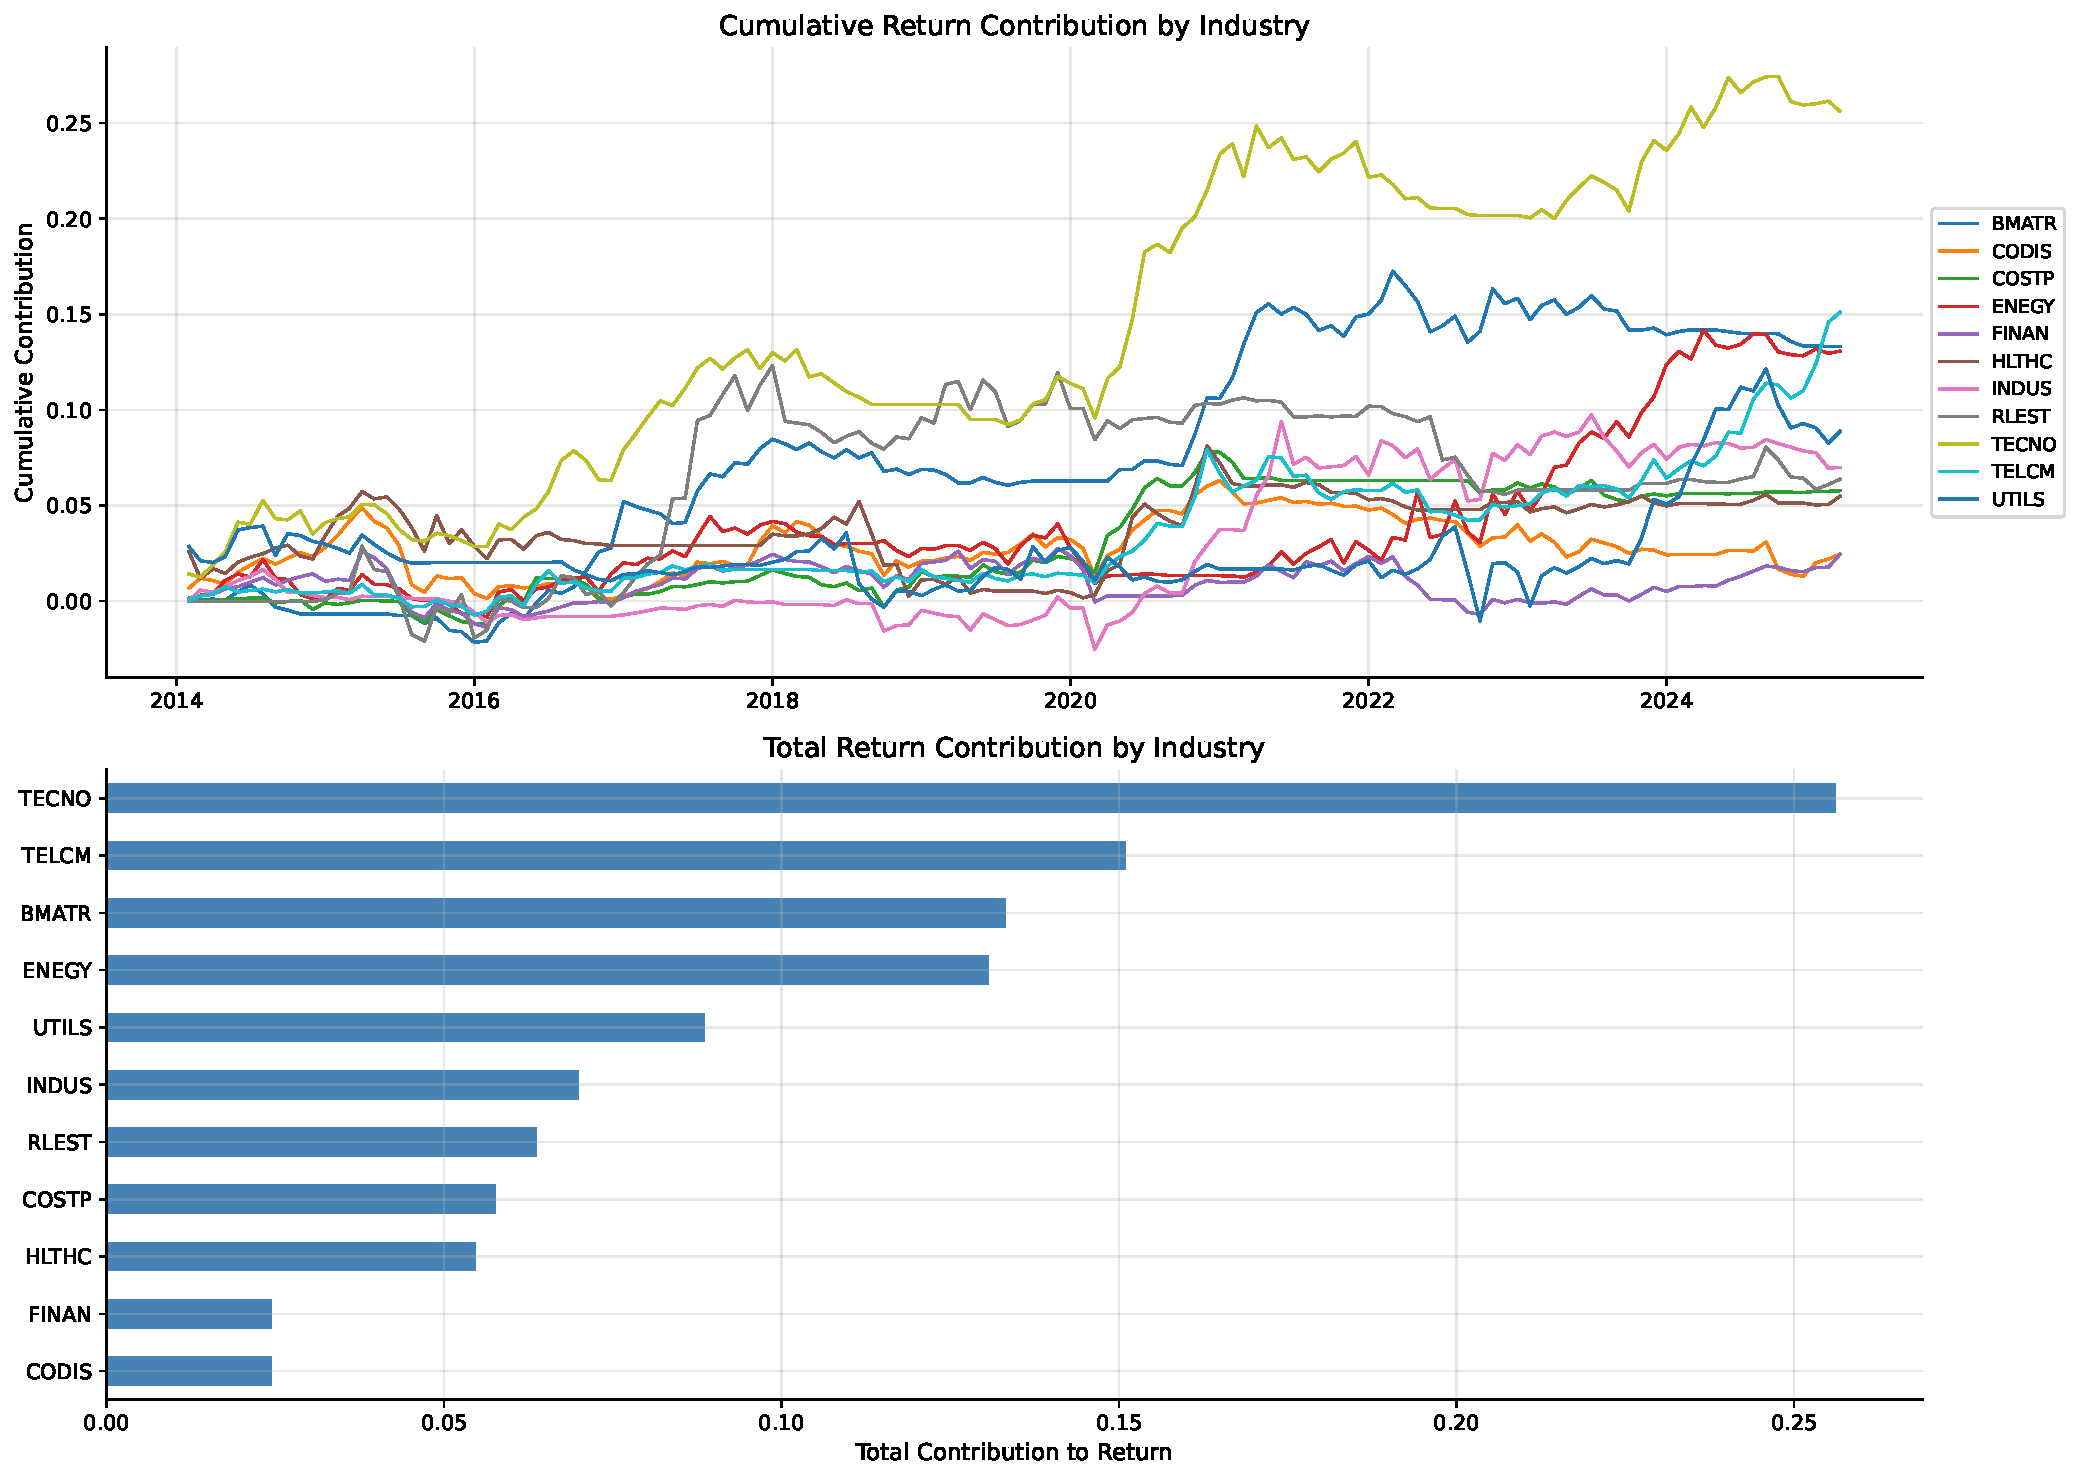
\includegraphics[width=0.85\textwidth]{nb08_return_decomposition.pdf}
    \caption{Return decomposition by industry: (top) cumulative contribution of each industry over time, (bottom) total contribution ranking.}
    \label{fig:decomp}
\end{figure}

\begin{figure}[H]
    \centering
    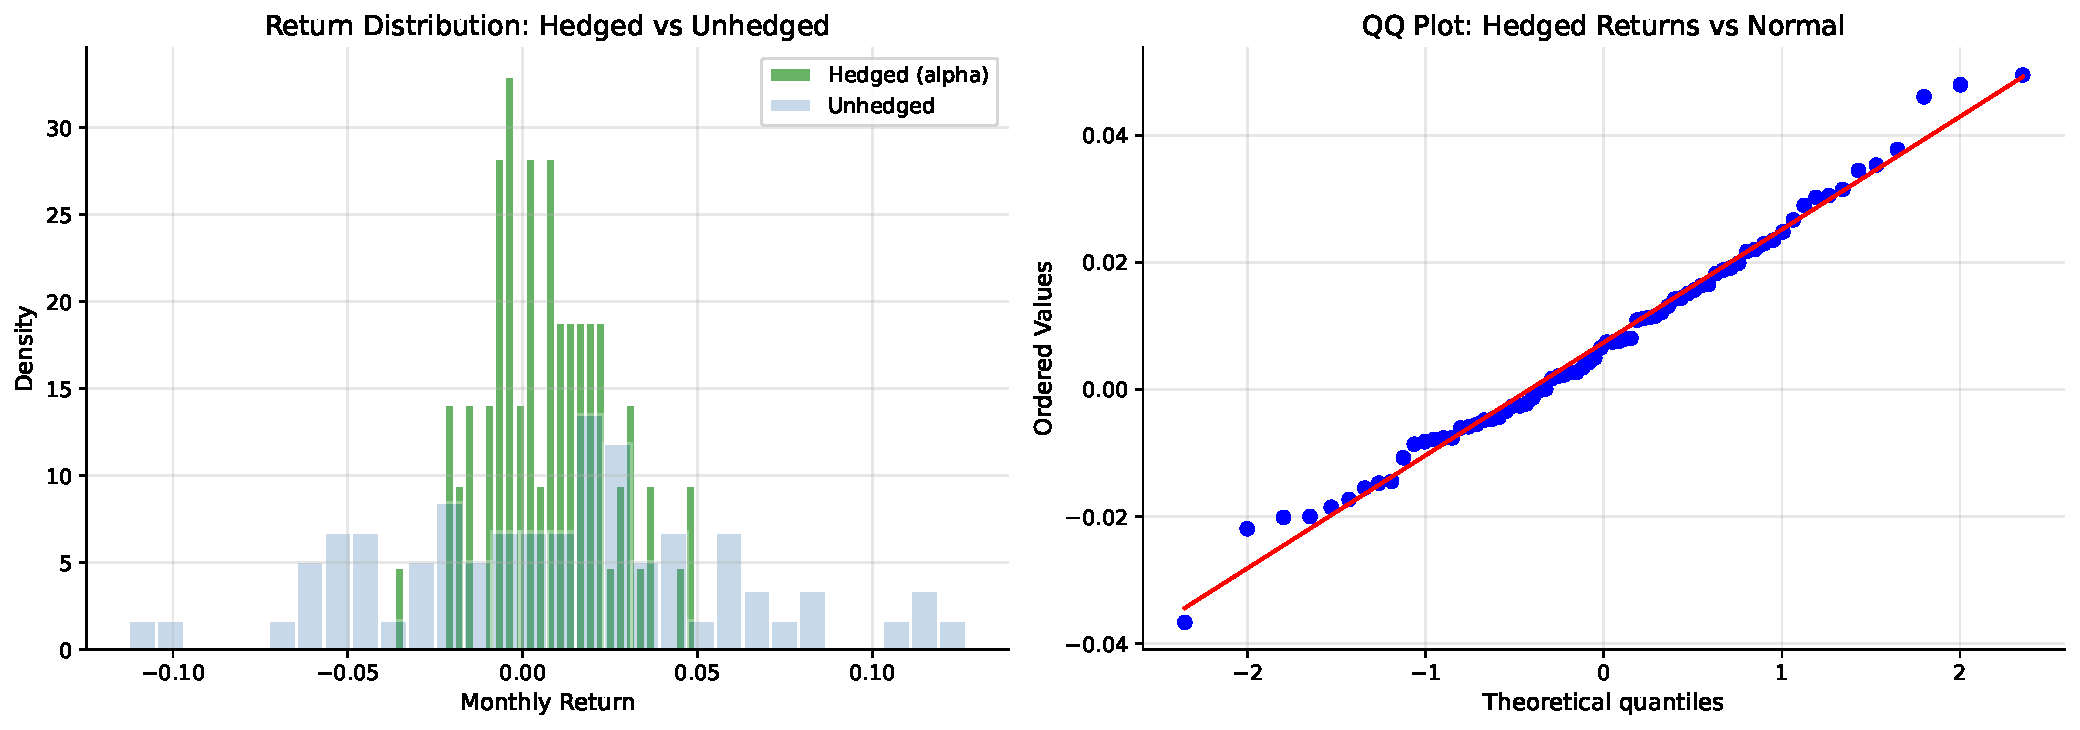
\includegraphics[width=0.85\textwidth]{nb09_return_dist.pdf}
    \caption{Monthly return distribution: (left) histogram of hedged vs.\ unhedged returns, (right) QQ plot of hedged returns vs.\ normal distribution.}
    \label{fig:return_dist}
\end{figure}

\end{document}
